\documentclass{ximera}

\begin{document}
	\author{Stitz-Zeager}
	\xmtitle{TITLE}


\mfpicnumber{1}

\opengraphsfile{TheInverseTrigonometricFunctions}

\setcounter{footnote}{0}

\label{TheInverseTrigonometricFunctions}

In this section we concern ourselves with finding inverses of the circular (trigonometric) functions.\footnote{We have already discussed this concept in Section \ref{AppRightTrig} as the `angle finder' in the context of acute angles in right triangles.}  Our immediate problem is that, owing to their periodic nature, none of the six circular functions is  one-to-one.  To remedy this, we restrict the domains of the circular functions in the same way we restricted the domain of the quadratic function in Example \ref{inverserestrictionex} in Section \ref{InverseFunctions} to obtain a one-to-one function.  

\smallskip


We start with $f(t)  = \sin(t)$ and restrict our domain to $\left[ -\frac{\pi}{2}, \frac{\pi}{2}\right]$ in order to keep the range as $[-1,1]$ as well as the properties of being smooth and continuous.

\smallskip


\begin{center}

\begin{mfpic}[15]{-13}{13}{-1.5}{1.5}
\axes
\point[4pt]{(-1.5708,-1), (0,0), (1.5708,1)}
\tlabel[cc](13,-0.5){\scriptsize $t$}
\tlabel[cc](0.5,1.5){\scriptsize $y$}
\tcaption{Restricting the domain of $f(t) = \sin(t)$ to $\left[-\frac{\pi}{2}, \frac{\pi}{2}\right]$.}
\ymarks{-1,1}
\dashed \arrow \reverse \arrow \function{-12, 12, 0.1}{sin(x)}
\penwd{1.25pt}
\function{-1.5708,1.5708, 0.1}{sin(x)}
\end{mfpic}

\end{center} 


\smallskip

Recall from Section \ref{InverseFunctions} that the inverse of a function $f$ is typically denoted $f^{-1}$.  For this reason, some textbooks use the notation $f^{-1}(t) = \sin^{-1}(t)$ for the inverse of $f(t) = \sin(t)$.  The obvious pitfall here is our convention of writing $(\sin(t))^2$ as $\sin^{2}(t)$, $(\sin(t))^3$ as $\sin^{3}(t)$ and so on.  It is far too easy to confuse $\sin^{-1}(t)$ with  $\frac{1}{\sin(t)} = \csc(t)$ so we will not use this notation in our text.\footnote{But be aware that many books do! As always, be sure to check the context!}

\smallskip

Instead, we use the notation $f^{-1}(t) = \arcsin(t)$, read `arc-sine of $t$'.  We'll explain the `arc' in `arcsine' shortly.  For now, we graph $f(t) = \sin(t)$ and $f^{-1}(t) = \arcsin(t)$, where we obtain the latter from the former by reflecting it across the line $y=t$, in accordance with Theorem \ref{inversefunctionprops}. \index{arcsine ! graph of}


\[ \begin{array}{ccc}

\begin{mfpic}[25]{-2}{2}{-2}{2}
\point[4pt]{(-1.5708,-1), (0,0), (1.5708,1)}
\axes
\tlabel[cc](2,-0.25){\scriptsize $t$}
\tlabel[cc](0.25,2){\scriptsize $y$}
\tcaption{\scriptsize $f(t) = \sin(t)$,  $-\frac{\pi}{2} \leq t \leq  \frac{\pi}{2}$.}
\xmarks{-1.5708, 1.5708}
\ymarks{-1,1}
\tlpointsep{4pt}
\axislabels {x}{{\scriptsize $-\frac{\pi}{2} \hspace{7pt}$} -1.5708, {\scriptsize $\frac{\pi}{2}$} 1.5708}
\axislabels {y}{{\scriptsize $-1$} -1, {\scriptsize $1$} 1}
\penwd{1.25pt}
\function{-1.5708,1.5708, 0.1}{sin(x)}
\end{mfpic}

&

\stackrel{\stackrel{\mbox{\scriptsize reflect across $y=t$}}{\xrightarrow{\hspace{1in}}}}{\mbox{ \scriptsize switch $t$ and $y$ coordinates}} 

&

\begin{mfpic}[25]{-2}{2}{-2}{2}
\point[4pt]{(-1,-1.5708), (0,0), (1,1.5708)}
\axes
\tlabel[cc](2,-0.25){\scriptsize $t$}
\tlabel[cc](0.25,2){\scriptsize $y$}
\tcaption{\scriptsize $f^{-1}(t) = \arcsin(t)$.}
\ymarks{-1.5708, 1.5708}
\xmarks{-1,1}
\tlpointsep{4pt}
\axislabels {y}{{\scriptsize $-\frac{\pi}{2}$} -1.5708, {\scriptsize $\frac{\pi}{2}$} 1.5708}
\axislabels {x}{{\scriptsize $-1 \hspace{7pt}$} -1, {\scriptsize $1$} 1}
\penwd{1.25pt}
\parafcn{-1.5708,1.5708, 0.1}{(sin(t),t)}
\end{mfpic}

\end{array}\]

Next, we consider $g(t) = \cos(t)$.  Here, we select the interval $[0,\pi]$ for our restriction.  
\begin{center}

\begin{mfpic}[15]{-13}{13}{-1.5}{1.5}
\axes
\point[4pt]{(0,1), (1.5708,0), (3.1416, -1)}
\tlabel[cc](13,-0.5){\scriptsize $t$}
\tlabel[cc](0.5,1.5){\scriptsize $y$}
\tcaption{Restricting the domain of $f(t) = \cos(t)$ to $[0,\pi]$.}
\ymarks{-1,1}
\dashed \arrow \reverse \arrow \function{-12.5664, 12.5664, 0.1}{cos(x)}
\penwd{1.25pt}
\function{0, 3.1416, 0.1}{cos(x)}
\end{mfpic}

\end{center} 

Reflecting the across the line $y = t$ produces  the graph $y = g^{-1}(t) = \arccos(t)$. \index{arccosine ! graph of}


\[ \begin{array}{ccc}
\begin{mfpic}[25]{-0.5}{4}{-2.25}{2.25}
\point[4pt]{(0,1), (1.5708,0), (3.1416, -1)}
\axes
\tlabel[cc](4,-0.25){\scriptsize $t$}
\tlabel[cc](0.25,2.25){\scriptsize $y$}
\tcaption{\scriptsize  $f(t) = \cos(t)$, $0 \leq t \leq \pi$}
\xmarks{1.5708, 3.1416}
\ymarks{-1,1}
\tlpointsep{4pt}
\axislabels {x}{{\scriptsize $\frac{\pi}{2}$} 1.5708,  {\scriptsize $\pi$} 3.1416}
\axislabels {y}{{\scriptsize $-1$} -1, { \scriptsize $1$} 1}
\penwd{1.25pt}
\function{0, 3.1416, 0.1}{cos(x)}
\end{mfpic}

&

\stackrel{\stackrel{\mbox{\scriptsize reflect across $y=t$}}{\xrightarrow{\hspace{1in}}}}{\mbox{ \scriptsize switch $t$ and $y$ coordinates}} 

&

\begin{mfpic}[25]{-2.25}{2.25}{-0.5}{4}
\point[4pt]{(1,0), (0,1.5708), (-1,3.1416)}
\axes
\tlabel[cc](2.25,-0.25){\scriptsize $t$}
\tlabel[cc](0.25,4){\scriptsize $y$}
\tcaption{\scriptsize $f^{-1}(t) = \arccos(t)$.}
\xmarks{-1,1}
\ymarks{1.5708, 3.1416}
\tlpointsep{4pt}
\axislabels {y}{{\scriptsize $\frac{\pi}{2}$} 1.5708,  {\scriptsize $\pi$} 3.1416}
\axislabels {x}{{\scriptsize $-1 \hspace{7pt}$} -1, {\scriptsize $1$} 1}
\penwd{1.25pt}
\parafcn{0, 3.1416, 0.1}{(cos(t), t)}
\end{mfpic}

\end{array}\]

We list some important facts about the arcsine and arccosine functions in the following theorem.\footnote{We switch the input variable to the arcsine and arccosine functions to `$x$' to avoid confusion with the outputs we label `$t$.'}   Everything in Theorem \ref{arccosinesinefunctionprops} is a direct consequence of Theorem \ref{inversefunctionprops} as applied to the (restricted) sine and cosine functions, and as such, its proof is left to the reader.

\smallskip

\colorbox{ResultColor}{\bbm

\begin{thm} \label{arccosinesinefunctionprops}  \textbf{Properties of the Arccosine and Arcsine Functions} \index{arccosine ! definition of} \index{arccosine ! properties of} \index{arcsine ! definition of} \index{arcsine ! properties of} 

\begin{itemize}

\item  Properties of $F(x) = \arcsin(x)$

\begin{itemize}
 
\item Domain:  $[-1,1]$

\item Range:  $\left[ -\frac{\pi}{2}, \frac{\pi}{2}\right]$

\item $\arcsin(x) = t$ if and only if $\sin(t) = x$ and $-\frac{\pi}{2} \leq t \leq \frac{\pi}{2}$

\item $\sin(\arcsin(x)) = x$ provided $-1 \leq x \leq 1$

\item $\arcsin(\sin(t)) = t$ provided $-\frac{\pi}{2} \leq t \leq \frac{\pi}{2}$ 

\item $F(x) = \arcsin(x)$ is odd

\end{itemize}

\item  Properties of $G(x)= \arccos(x)$

\begin{itemize}

\item Domain:  $[-1,1]$

\item Range:  $[0,\pi]$

\item $\arccos(x) = t$ if and only if  $\cos(t) = x$ and $0 \leq t \leq \pi$

\item $\cos(\arccos(x)) = x$ provided $-1 \leq x \leq 1$

\item $\arccos(\cos(t)) = t$ provided $0 \leq t \leq \pi$

\end{itemize}

\end{itemize}

\end{thm}

\smallskip

\ebm}

\smallskip

Before moving to an example, we take a moment to understand the `arc' in `arcsine.'  Consider the figure below which illustrates the specific case of $\arcsin\left(\frac{\sqrt{3}}{2} \right)$. 

\smallskip

By definition, the real number $t = \arcsin\left(\frac{\sqrt{3}}{2} \right)$ satisfies $\sin(t) =  \frac{\sqrt{3}}{2}$ with $-\frac{\pi}{2} \leq t \leq \frac{\pi}{2}$.  In other words, we are looking for angle measuring $t$ radians between $-\frac{\pi}{2}$ and $\frac{\pi}{2}$ with a sine of $\frac{\sqrt{3}}{2}$. Hence, $\arcsin\left(\frac{\sqrt{3}}{2} \right) = \frac{\pi}{3}$. 

\smallskip

In terms of oriented arcs\footnote{See page \pageref{wrappingfunction} if you need a review of how we associate real numbers with angles in radian measure.}, if we start at $(1,0)$  and travel along the Unit Circle in the positive (counterclockwise) direction for $\frac{\pi}{3}$ units, we will arrive at the point whose $y$-coordinate is  $\frac{\sqrt{3}}{2}$.   Hence,  the real number $\frac{\pi}{3}$ also corresponds to  `arc' corresponding to the `sine' that is $\frac{\sqrt{3}}{2}$.

\smallskip

\smallskip

\phantomsection
\label{arcinarcsine}

\begin{center}
\begin{tabular}{cc}

\begin{mfpic}[18]{-5}{5}{-5}{5}
\axes
\tlabel(5,-0.5){\scriptsize $x$}
\tlabel(0.5,5){\scriptsize $y$}
\tlabel(3.1,-0.75){\scriptsize $1$}
\tlabel(0.25,3.1){\scriptsize $1$}
\xmarks{-3 step 3 until 3}
\ymarks{-3 step 3 until 3}
\tlabel[cc](2.75, 2.6){\scriptsize $\left( \frac{1}{2}, \frac{\sqrt{3}}{2} \right)$}
\drawcolor[gray]{0.7}
\circle{(0,0),3}
\drawcolor{black}
%\arrow \polyline{(5, 0), (0,0), (2.5, 4.3301)}
%\arrow \parafcn{5, 55, 5}{1.5*dir(t)}
\point[3pt]{(0,0), (1.5, 2.6)}
\end{mfpic} 

&

\begin{mfpic}[18]{-5}{5}{-5}{5}
\axes
\tlabel(5,-0.5){\scriptsize $x$}
\tlabel(0.5,5){\scriptsize $y$}
\tlabel(3.1,-0.75){\scriptsize $1$}
\tlabel(0.25,3.1){\scriptsize $1$}
\xmarks{-3 step 3 until 3}
\ymarks{-3 step 3 until 3}
\drawcolor[gray]{0.7}
\circle{(0,0),3}
\drawcolor{black}
\arrow \polyline{(0,0), (2.5, 4.3301)}
\arrow \parafcn{5, 55, 5}{1.5*dir(t)}
\tlabel[cc](1.732, 1){\scriptsize $\frac{\pi}{3}$}
\penwd{1.25pt}
\arrow \parafcn{0,60,5}{3*dir(t)}
\tlabel[cc](4.25,1.75){\scriptsize $\arcsin \left( \frac{\sqrt{3}}{2} \right)  = \frac{\pi}{3}$}
\point[3pt]{(0,0), (1.5, 2.6)}
\end{mfpic} 



\\

$y$-value on Unit Circle is $\frac{\sqrt{3}}{2}$.

&

corresponding oriented arc:  $t = \frac{\pi}{3}$



 \\


\end{tabular}

\end{center}


\smallskip


In general, the function $f(t) = \sin(t)$ takes a real number input $t$, associates it with the angle $\theta = t$ radians, and returns the value $\sin(\theta)$.  The value $\sin(\theta) = \sin(t)$ is the $y$-coordinate of the terminal point on the Unit Circle of an oriented arc of length $|t|$ whose initial point is $(1, 0)$.   

\smallskip

Hence, we may view the inputs to $f(t) = \sin(t)$ as oriented arcs and the outputs as $y$-coordinates on the Unit Circle.  Therefore, the function $f^{-1}$ reverses this process and takes $y$-coordinates on the Unit Circle and return oriented arcs, hence the `arc' in arcsine. 

\smallskip



 It is high time for an example.

\begin{ex}  \label{arccosinesineex} $~$

\begin{enumerate}  

\item Find the exact values of the following.

\begin{multicols}{2}

\begin{enumerate}

\item  $\arcsin\left(\frac{\sqrt{2}}{2}\right)$
\item  $\arccos\left(\frac{1}{2}\right)$ \vphantom{$\arcsin\left(\frac{\sqrt{2}}{2}\right)$}


\setcounter{HW}{\value{enumii}}

\end{enumerate}

\end{multicols}

\begin{multicols}{2}

\begin{enumerate}

\setcounter{enumii}{\value{HW}}

\item  $\arcsin\left(-\frac{1}{2}\right)$
\item  $\arccos\left(-\frac{\sqrt{2}}{2}\right)$


\setcounter{HW}{\value{enumii}}

\end{enumerate}

\end{multicols}

\begin{multicols}{2}

\begin{enumerate}

\setcounter{enumii}{\value{HW}}

\item  $\arccos\left( \cos\left(\frac{\pi}{6}\right)\right)$
\item  $\arccos\left( \cos\left(\frac{11\pi}{6}\right)\right)$

\setcounter{HW}{\value{enumii}}

\end{enumerate}

\end{multicols}

\begin{multicols}{2}

\begin{enumerate}

\setcounter{enumii}{\value{HW}}

\item  $\cos\left(\arccos\left(-\frac{3}{5}\right)\right)$
\item  $\sin\left(\arccos\left(-\frac{3}{5}\right)\right)$

\end{enumerate}

\end{multicols}

\item  \label{algarcsincos} Rewrite each of the following composite functions as algebraic functions of $x$ and state the domain.

\begin{multicols}{2}

\begin{enumerate}

\item \label{tanarccos} $f(x) = \tan\left(\arccos\left(x \right)\right)$

\item  \label{cosarcsin} $g(x) = \cos\left(2 \arcsin(x)\right)$

\end{enumerate}

\end{multicols}

\end{enumerate}

{\bf Solution.}

The best way to approach these problems is to remember that $\arcsin(x)$ and $\arccos(x)$ are real numbers which correspond to the radian measure of angles that fall within a certain prescribed range.

\begin{enumerate}

\item 

\begin{enumerate}

\item  To find $\arcsin\left(\frac{\sqrt{2}}{2}\right)$, we need the angle measuring $t$ radians which lies between $-\frac{\pi}{2}$ and $\frac{\pi}{2}$ with $\sin(t) = \frac{\sqrt{2}}{2}$. Hence, $\arcsin\left(\frac{\sqrt{2}}{2}\right) = \frac{\pi}{4}$.

\item  To find $\arccos\left(\frac{1}{2}\right)$, we are looking for the angle measuring $t$ radians which lies between $0$ and $\pi$ that has  $\cos(t) = \frac{1}{2}$.   Our answer is $\arccos\left(\frac{1}{2}\right)= \frac{\pi}{3}$.

\item  For  $\arcsin\left(-\frac{1}{2}\right)$,  we are looking for an angle measuring $t$ radians which lies between $-\frac{\pi}{2}$ and $\frac{\pi}{2}$ with $\sin(t) = -\frac{1}{2}$. Hence,  $\arcsin\left(-\frac{1}{2}\right) = -\frac{\pi}{6}$.

\smallskip

Alternatively, we could use the fact that the arcsine function is odd, so $\arcsin\left(-\frac{1}{2}\right) = - \arcsin\left(\frac{1}{2}\right)$.

\smallskip

We find  $\arcsin\left(\frac{1}{2}\right) = \frac{\pi}{6}$, so $\arcsin\left(-\frac{1}{2}\right) = - \arcsin\left(\frac{1}{2}\right) = -\frac{\pi}{6}$.


\item  For $\arccos\left(-\frac{\sqrt{2}}{2}\right)$, we need the angle measuring $t$ radians which lies between $0$ and $\pi$ with $\cos(t) = -\frac{\sqrt{2}}{2}$  .  Hence, $\arccos\left(-\frac{\sqrt{2}}{2}\right) = \frac{3\pi}{4}$.


\item  Since $0 \leq \frac{\pi}{6} \leq \pi$, we could simply invoke Theorem \ref{arccosinesinefunctionprops} to get $\arccos\left( \cos\left(\frac{\pi}{6}\right)\right) = \frac{\pi}{6}$.  

\smallskip

However, in order to make sure we understand \textit{why} this is the case, we choose to work the example through using the definition of arccosine.  

\smallskip

Working from the inside out,  $\arccos\left( \cos\left(\frac{\pi}{6}\right)\right) = \arccos\left( \frac{\sqrt{3}}{2}\right)$.  To find $\arccos\left( \frac{\sqrt{3}}{2}\right)$, we need an angle measuring  $t$ radians which lies between $0$ and $\pi$ that has $\cos(t) = \frac{\sqrt{3}}{2}$.   We get $t = \frac{\pi}{6}$, so that  $\arccos\left( \cos\left(\frac{\pi}{6}\right)\right) =  \arccos\left( \frac{\sqrt{3}}{2}\right) = \frac{\pi}{6}$.

\item Since $\frac{11\pi}{6}$ does not fall between $0$ and $\pi$, Theorem \ref{arccosinesinefunctionprops} does not apply.  We are forced to work through from the inside out starting with  $\arccos\left( \cos\left(\frac{11\pi}{6}\right)\right) = \arccos\left(\frac{\sqrt{3}}{2}\right)$.  From the previous problem, we know $\arccos\left(\frac{\sqrt{3}}{2}\right) = \frac{\pi}{6}$.  Hence,  $\arccos\left( \cos\left(\frac{11\pi}{6}\right)\right) = \frac{\pi}{6}$.

\item  One way to simplify  $\cos\left(\arccos\left(-\frac{3}{5}\right)\right)$ is to use Theorem \ref{arccosinesinefunctionprops} directly.  Since $-\frac{3}{5}$ is between $-1$ and $1$, we have that $\cos\left(\arccos\left(-\frac{3}{5}\right)\right) = -\frac{3}{5}$ and we are done.  

\smallskip

However, as before, to really understand \textit{why} this cancellation occurs, we  let $t = \arccos\left(-\frac{3}{5}\right)$.  By definition,  $\cos(t) = -\frac{3}{5}$. Hence, $\cos\left(\arccos\left(-\frac{3}{5}\right)\right) = \cos(t) = -\frac{3}{5}$, and we are finished in (nearly) the same amount of time.

\item  As in the previous example, we let $t = \arccos\left(-\frac{3}{5}\right)$ so that  $\cos(t) = -\frac{3}{5}$ for some angle measuring $t$  radians between $0$ and $\pi$.

\smallskip

Since $\cos(t) < 0$,  we can narrow this down a bit and conclude that $\frac{\pi}{2} < t < \pi$, so that $t$ corresponds to an angle in Quadrant II. 

\smallskip

In terms of $t$, then, we need to find $\sin\left(\arccos\left(-\frac{3}{5}\right)\right) = \sin(t)$, and since we know $\cos(t)$, the fastest route is through the Pythagorean Identity.  

\smallskip 

We get $\sin^{2}(t) = 1 - \cos^{2}(t) = 1 - \left(-\frac{3}{5}\right)^2 = \frac{16}{25}$.  Since $t$ corresponds to a Quadrant II angle, we choose the positive root, $\sin(t) = \frac{4}{5}$, so $\sin\left(\arccos\left(-\frac{3}{5}\right)\right) = \frac{4}{5}$.

\end{enumerate}

\item

\begin{enumerate}

\item We begin this problem in the same manner we began the previous two problems.  We let  $t = \arccos(x)$, so our goal is to find a way to express $\tan\left(\arccos\left(x \right)\right) = \tan(t)$ in terms of $x$.  

\smallskip

Since $t = \arccos(x)$, we know $\cos(t) = x$ where $0 \leq t \leq \pi$.   One approach\footnote{Alternatively, we could use the identity:  $1 + \tan^{2}(t) = \sec^{2}(t)$.  Since $x = \cos(t)$,  $\sec(t) = \frac{1}{\cos(t)} = \frac{1}{x}$.  The reader is invited to work through this approach to see what, if any, difficulties arise.} to finding $\tan(t)$ is to use the quotient identity $\tan(t) = \frac{\sin(t)}{\cos(t)}$.  Since we know $\cos(t)$, we just need to find $\sin(t)$.

\smallskip

Using the Pythagorean Identity, we get  $\sin^{2}(t) = 1 - \cos^{2}(t) = 1 - x^2$ so that $\sin(t) = \pm \sqrt{1-x^2}$.  Since $0 \leq t \leq \pi$,   $\sin(t) \geq 0$, so we choose $\sin(t) = \sqrt{1-x^2}$.  

\smallskip

Thus, $\tan(t) = \frac{\sin(t)}{\cos(t)} = \frac{\sqrt{1-x^2}}{x}$, so $f(x) = \tan(\arccos(x)) =  \frac{\sqrt{1-x^2}}{x}$.

\smallskip

To determine the domain, we harken back to Section \ref{FunctionComposition}.  The function $f(x) = \tan\left(\arccos\left(x \right)\right)$ can be thought of as a two step process:  first, take the arccosine of a number, and second, take the tangent of whatever comes out of the arccosine.

\smallskip

Since the domain of $\arccos(x)$ is $-1 \leq x \leq 1$, the domain of $f$ will be some subset of $[-1,1]$.  The range of  $\arccos(x)$ is $[0,\pi]$, and of these values, only  $\frac{\pi}{2}$ will cause a problem for the tangent function.  Since $\arccos(x) = \frac{\pi}{2}$ happens when $x = \cos\left(\frac{\pi}{2} \right) = 0$, we exclude $x=0$ from our domain.  Hence, the domain of  $f(x) = \tan\left(\arccos\left(x \right)\right) =\frac{\sqrt{1-x^2}}{x}$  is  $[-1,0)\cup(0,1]$.  

\smallskip

Note that \textit{in this particular case}, we could have obtained the correct domain of $f$ using its algebraic description:  $f(x) = \tan(\arccos(x)) =  \frac{\sqrt{1-x^2}}{x}$.  This is not always true, however, as we'll see in the next problem.

\item We proceed as in the previous problem by writing $t = \arcsin(x)$ so that $t$ lies in the interval $\left[ -\frac{\pi}{2}, \frac{\pi}{2}\right]$ with $\sin(t) = x$.  We aim to express $\cos\left(2 \arcsin(x)\right) = \cos(2t)$ in terms of $x$.  

\smallskip

Thanks to Theorem \ref{doubleangle}, we have three choices for rewriting $\cos(2t)$:  $\cos(2t) = \cos^{2}(t) - \sin^{2}(t)$, $ \cos(2t) = 2\cos^{2}(t) - 1$ and $\cos(2t) = 1 - 2\sin^{2}(t)$.  

\smallskip

Since we know $x = \sin(t)$, we choose: $\cos\left(2 \arcsin(x)\right) = \cos(2t)  = 1 - 2\sin^{2}(t) = 1 - 2x^2$.  Hence, $g(x) = \cos\left(2 \arcsin(x)\right) = 1 - 2x^2$.

\smallskip

To find the domain of $g(x) = \cos\left(2 \arcsin(x)\right)$, we once again appeal to what we learned in Section \ref{FunctionComposition}.  The domain of $\arcsin(x)$ is  $[-1,1]$, and since there are no domain restrictions on cosine, the domain of $g$ is $[-1,1]$.  
\smallskip

It is important to note that in this case, even though the algebraic expression $1-2x^2$ is defined for all real numbers, the domain of $g$ is limited to that of $\arcsin(x)$, namely $[-1,1]$. The adage `find the domain \textit{before} you simplify' rings as true here as it did in Chapter \ref{FurtherTopicsonFunctions}. \qed

\end{enumerate}

\end{enumerate}

\end{ex}



\smallskip

The next pair of functions we wish to discuss are the inverses of tangent and cotangent.  First, we restrict $f(t) = \tan(t)$ to its fundamental cycle on $\left(-\frac{\pi}{2}, \frac{\pi}{2}\right)$ to obtain the arctangent function, $f^{-1}(t) = \arctan(t)$. Among other things, note that the \textit{vertical} asymptotes $t = -\frac{\pi}{2}$ and $t = \frac{\pi}{2}$ of the graph of $f(t) = \tan(t)$ become the \textit{horizontal} asymptotes $y = -\frac{\pi}{2}$ and $y = \frac{\pi}{2}$ of the graph of $f^{-1}(t) = \arctan(t)$.  \index{arctangent ! graph of}

\[ \begin{array}{ccc}

\begin{mfpic}[25][20]{-2}{2}{-4}{4}
\point[4pt]{(-0.7854,-1), (0,0), (0.7854,1)}
\axes
\tlabel[cc](2,-0.25){\scriptsize $t$}
\tlabel[cc](0.25,4){\scriptsize $y$}
\tcaption{\scriptsize $f(t) = \tan(t)$,  $-\frac{\pi}{2} < t <  \frac{\pi}{2}$.}
\xmarks{-0.7854, 0.7854}
\ymarks{-1,1}
\tlpointsep{4pt}
\axislabels {x}{{\scriptsize $-\frac{\pi}{4} \hspace{7pt}$} -0.7854, {\scriptsize $-\frac{\pi}{2} \hspace{7pt}$} -1.5708, {\scriptsize $\frac{\pi}{4}$} 0.7854, {\scriptsize $\frac{\pi}{2}$} 1.5708}
\axislabels {y}{{\scriptsize $-1$} -1, {\scriptsize $1$} 1}
\dashed \polyline{(1.5708,-4), (1.5708,4)}
\dashed \polyline{(-1.5708,-4), (-1.5708,4)}
\penwd{1.25pt}
\arrow \reverse \arrow \function{-1.3181, 1.3181, 0.1}{tan(x)}
\end{mfpic}

&

\stackrel{\stackrel{\mbox{\scriptsize reflect across $y=t$}}{\xrightarrow{\hspace{1in}}}}{\mbox{ \scriptsize switch $t$ and $y$ coordinates}} 

&

\begin{mfpic}[20][25]{-4}{4}{-2}{2}
\point[4pt]{(-1, -0.7854), (0,0), (1,0.7854)}
\axes
\tlabel[cc](4,-0.25){\scriptsize $t$}
\tlabel[cc](0.25,2){\scriptsize $y$}
\tcaption{\scriptsize $f^{-1}(t) = \arctan(t)$.}
\ymarks{-0.7854, 0.7854}
\xmarks{-1,1}
\tlpointsep{4pt}
\axislabels {y}{{\scriptsize $-\frac{\pi}{4}$} -0.7854, {\scriptsize $-\frac{\pi}{2}$} -1.5708, {\scriptsize $\frac{\pi}{4}$} 0.7854, {\scriptsize $\frac{\pi}{2}$} 1.5708}
\axislabels {x}{{\scriptsize $-1 \hspace{7pt}$} -1, {\scriptsize $1$} 1}
\dashed \polyline{(-4, 1.5708), (4, 1.5708)}
\dashed \polyline{(-4, -1.5708), (4, -1.5708)}
\penwd{1.25pt}
\arrow \reverse \arrow \parafcn{-1.3181, 1.3181, 0.1}{(tan(t), t)}
\end{mfpic}

\end{array}\]

Next, we restrict $g(t) = \cot(t)$ to its fundamental cycle on $(0,\pi)$ to obtain $g^{-1}(t) = \mbox{arccot}(t)$, the arccotangent function.  Once again, the vertical asymptotes $t=0$ and $t=\pi$ of the graph of $g(t) = \cot(t)$ become the horizontal asymptotes $y = 0$ and $y = \pi$ of the graph of $g^{-1}(t) = \mbox{arccot}(t)$.  
\[ \begin{array}{ccc}

\begin{mfpic}[25][20]{-1}{4}{-4}{4.25}
\point[4pt]{ (0.7854,1), (1.5708,0), (2.3562,-1)}
\dashed \polyline{(3.1416,-4), (3.1416,4)}
\axes
\tlabel[cc](4,-0.25){\scriptsize $t$}
\tlabel[cc](0.25,4.25){\scriptsize $y$}
\tcaption{\scriptsize $g(t) = \cot(t)$, $0 < t < \pi$.}
\xmarks{0.7854, 1.5708, 2.3562, 3.1416}
\ymarks{-1,1}
\tlpointsep{4pt}
\axislabels {x}{{\scriptsize $\frac{\pi}{4}$} 0.7854, {\scriptsize $\frac{\pi}{2}$} 1.5708, {\scriptsize $\frac{3\pi}{4}$} 2.3562, {\scriptsize $\pi$} 3.1416}
\axislabels {y}{{\scriptsize $-1$} -1, {\scriptsize $1$} 1}
\penwd{1.25pt}
\arrow \reverse \arrow \function{0.2450, 2.8966, 0.1}{cot(x)}
\end{mfpic}

&

\stackrel{\stackrel{\mbox{\scriptsize reflect across $y=t$}}{\xrightarrow{\hspace{1in}}}}{\mbox{ \scriptsize switch $t$ and $y$ coordinates}} 

&

\begin{mfpic}[20][25]{-4}{4.25}{-1}{4}
\point[4pt]{ (1,0.7854), (0,1.5708), (-1,2.3562)}
\dashed \polyline{(-4,3.1416), (4,3.1416)}
\axes
\tlabel[cc](4.25,-0.25){\scriptsize $t$}
\tlabel[cc](0.25,4){\scriptsize $y$}
\tcaption{\scriptsize $g^{-1}(t) = \mbox{arccot}(t)$.}
\ymarks{0.7854, 1.5708, 2.3562, 3.1416}
\xmarks{-1,1}
\tlpointsep{4pt}
\axislabels {y}{{\scriptsize $\frac{\pi}{4}$} 0.7854, {\scriptsize $\frac{\pi}{2}$} 1.5708, {\scriptsize $\frac{3\pi}{4}$} 2.3562, {\scriptsize $\pi$} 3.1416}
\axislabels {x}{{\scriptsize $-1 \hspace{7pt}$} -1, {\scriptsize $1$} 1}
\penwd{1.25pt}
\arrow \reverse \arrow \parafcn{0.2450, 2.8966, 0.1}{(cot(t),t)}
\end{mfpic}

\end{array}\] \index{arccotangent ! graph of}

Below we summarize the important properties of the arctangent and arccotangent functions.

\smallskip


\colorbox{ResultColor}{\bbm

\begin{thm} \label{arctangentcotangentfunctionprops}  \textbf{Properties of the Arctangent and Arccotangent Functions} \index{arctangent ! definition of} \index{arctangent ! properties of} \index{arccotangent ! definition of} \index{arccotangent ! properties of} 

\begin{itemize}

\item Properties of $F(x)= \arctan(x)$

\begin{itemize}

\item Domain: $(-\infty, \infty)$

\item Range: $\left(-\frac{\pi}{2}, \frac{\pi}{2}\right)$

\item  $\ds{\lim_{x \rightarrow -\infty} \arctan(x)}$ $= -\frac{\pi}{2}$;  $\ds{\lim_{x \rightarrow \infty} \arctan(x)}$ $=\frac{\pi}{2}$

\item  $\arctan(x) = t$ if and only if $\tan(t) = x$ and $-\frac{\pi}{2} < t < \frac{\pi}{2}$ 

\item  $\arctan(x) = \mbox{arccot}\left(\frac{1}{x}\right)$ for $x > 0$

\item  $\tan\left(\arctan(x)\right) = x$ for all real numbers $x$

\item  $\arctan(\tan(t)) = t$ provided $-\frac{\pi}{2} < t < \frac{\pi}{2}$

\item $F(x)= \arctan(x)$ is odd

\end{itemize}

\item Properties of $G(x) = \mbox{arccot}(x)$

\begin{itemize}

\item Domain: $(-\infty, \infty)$

\item Range: $(0, \pi)$

\item  $\ds{\lim_{x \rightarrow -\infty} \mbox{arccot}(x) =\pi}$; $\ds{\lim_{x \rightarrow \infty} \mbox{arccot}(x) = 0}$

\item  $\mbox{arccot}(x) = t$ if and only if $\cot(t) = x$ and $0 <  t < \pi$ 

\item  $\mbox{arccot}(x) =\arctan\left(\frac{1}{x}\right)$ for $x > 0$

\item  $\cot\left(\mbox{arccot}(x)\right) = x$ for all real numbers $x$

\item  $\mbox{arccot}(\cot(t)) = t$ provided $0 < t < \pi$

\end{itemize}

\end{itemize}

\end{thm}

\smallskip

\ebm}

\smallskip

The properties listed in Theorem \ref{arctangentcotangentfunctionprops} are consequences of the definitions of the arctangent and arccotangent functions along with Theorem \ref{inversefunctionprops}, and its proof is left to the reader.

\begin{ex} \label{arctanarccotexample} $~$

\begin{enumerate}

\item  Find the exact values of the following.

\begin{multicols}{2}

\begin{enumerate}

\item $\arctan(\sqrt{3})$
\item  $\mbox{arccot}(-\sqrt{3})$

\setcounter{HW}{\value{enumii}}

\end{enumerate}

\end{multicols}

\begin{multicols}{2}

\begin{enumerate}

\setcounter{enumii}{\value{HW}}

\item  $\cot(\mbox{arccot}(-5))$
\item  $\sin\left(\arctan\left(-\frac{4}{3}\right)\right)$

\end{enumerate}

\end{multicols}

\pagebreak

\item  Rewrite each of the following composite functions as algebraic functions of $x$ and state the domain.

\begin{multicols}{2}

\begin{enumerate}

\item  $\tan(2 \arctan(x))$

\item  \label{cosineofarccotex} $\cos(\mbox{arccot}(2x))$ 

\end{enumerate}

\end{multicols}

\end{enumerate}

{\bf Solution.}

\begin{enumerate}

\item

\begin{enumerate}

\item  To find $\arctan(\sqrt{3})$, we need the angle measuring $t$ radians which lies between $-\frac{\pi}{2}$ and $\frac{\pi}{2}$ with $\tan(t) = \sqrt{3}$.  We find  $\arctan(\sqrt{3}) = \frac{\pi}{3}$.

\item To find $\mbox{arccot}(-\sqrt{3})$, we need the angle measuring $t$ radians which lies between $0$ and $\pi$ with $\cot(t) = -\sqrt{3}$.  Hence, $\mbox{arccot}(-\sqrt{3}) = \frac{5\pi}{6}$.

\item  We can apply Theorem \ref{arctangentcotangentfunctionprops} directly and obtain $\cot(\mbox{arccot}(-5)) = -5$.  However, working it through provides us with yet another opportunity to understand why this is the case. 

\smallskip

Letting $t = \mbox{arccot}(-5)$,  by definition, $\cot(t)=-5$.  Hence, $\cot(\mbox{arccot}(-5)) = \cot(t)=-5$.

\item   We start simplifying  $\sin\left(\arctan\left(-\frac{4}{3}\right)\right)$ by letting $t = \arctan\left(-\frac{4}{3}\right)$.  By definition,  $\tan(t) = -\frac{4}{3}$ for some angle measuring $t$ radians which lies between $-\frac{\pi}{2}$ and $\frac{\pi}{2}$.   Since $\tan(t) < 0$, we know, in fact, $t$ corresponds to a Quadrant IV angle.  

\smallskip

We are given $\tan(t)$ but wish to know $\sin(t)$.  Since there is no direct identity to marry the two, we make a quick sketch of the situation below.  Since $\tan(t) = -\frac{4}{3} = \frac{-4}{3}$, we take $P(3,-4)$ as a point on the terminal side of $\theta = t =  \arctan\left(-\frac{4}{3}\right)$ radians.

\smallskip



\begin{center}


\begin{mfpic}[18]{-5}{5}{-5}{5}
\axes
\tlabel(4.75,-0.5){\scriptsize $x$}
\tlabel(0.25,4.5){\scriptsize $y$}
\tlabel(2.5,-2.75){\scriptsize $P(3,-4)$}
\tlabel[cc](1,-2.5){\scriptsize $r=5$}
\tlabel[cc](1.75,-1){\scriptsize $\theta$}
\xmarks{-2.68, -2,  -1.34, -0.67, 0.67, 1.34, 2, 2.68}
\ymarks{-2.68, -2,  -1.34, -0.67, 0.67, 1.34, 2, 2.68}
\tcaption{$P(3,-4)$ is on the terminal side of $\theta$.}
\drawcolor[gray]{0.7}
\circle{(0,0),3.354}
\drawcolor{black}
\arrow  \parafcn{-5, -50, -5}{1.5*dir(t)}
\penwd{1.25pt}
\arrow \reverse \arrow \polyline{(5,0),(0,0), (3, -4)}
\point[4pt]{(0,0), (2.012, -2.683)}
\tlpointsep{4pt}
\scriptsize 
\axislabels {x}{ {$-3 \hspace{7pt}$} -2, {$-1 \hspace{7pt}$} -0.67,  {$1$} 0.67,  {$3$} 2, {$-2 \hspace{7pt}$} -1.34, {$-4 \hspace{7pt}$} -2.68,  {$4$} 2.68}
\axislabels {y}{ {$-2$} -1.34, {$-4$} -2.68, {$2$} 1.34, {$4$} 2.68,  {$1$} 0.67,  {$3$} 2,  {$-1$} -0.67,  {$-3$} -2 }
\normalsize
\end{mfpic}

\end{center}

\smallskip

We find $r = \sqrt{x^2+y^2} = \sqrt{(3)^2+(-4)^2} = 5$, so $\sin(t) = -\frac{4}{5}$.  Hence, $\sin\left(\arctan\left(-\frac{4}{3}\right)\right) = -\frac{4}{5}$.

\end{enumerate}

\item  

\begin{enumerate}

\item We proceed as above and let $t = \arctan(x)$.  We have $\tan(t) = x$ where $-\frac{\pi}{2} < t < \frac{\pi}{2}$.   Our goal is to express  $\tan(2 \arctan(x)) = \tan(2t)$ in terms of $x$.  

\smallskip

From Theorem \ref{doubleangle}, we know  $\tan(2t) = \frac{2 \tan(t)}{1 - \tan^{2}(t)} = \frac{2x}{1-x^2}$.  Hence $f(x) = \tan(2 \arctan(x)) = \frac{2x}{1-x^2}$.   

\smallskip

To find the domain, we once again think of $f(x) = \tan(2 \arctan(x))$ as a  sequence of steps and work from the inside out.

\smallskip

The first step is to find the arctangent of a real number.  Since the domain of $\arctan(x)$ is all real numbers, we have no restrictions here and we get out all values $\left(-\frac{\pi}{2}, \frac{\pi}{2} \right)$.

\smallskip

The next step is to multiply $\arctan(x)$ by $2$.  There are no restrictions here, either.   Since the range of $\arctan(x)$ is $\left(-\frac{\pi}{2}, \frac{\pi}{2} \right)$, the range of $2 \arctan(x)$ is $(-\pi, \pi)$.  

\smallskip

The last step is to take the tangent of $2 \arctan(x)$.  Since we are taking the tangent of values in the interval $(-\pi, \pi)$,   we will run into trouble if $2 \arctan(x) = \pm \frac{\pi}{2}$, that is,  if $\arctan(x) = \pm \frac{\pi}{4}$. Since this happens exactly when $x = \tan\left( \pm \frac{\pi}{4}\right) = \pm 1$, we must exclude $x = \pm 1$ from the domain of $f$.

\smallskip

Hence, the domain of   $f(x) = \tan(2 \arctan(x))$ is  $(-\infty, -1) \cup (-1,1) \cup (1,\infty)$. In this example, we could have obtained the correct answer by looking at the algebraic equivalence, $f(x) =  \frac{2x}{1-x^2}$.  However, as we saw in Example \ref{arccosinesineex}, number \ref{cosarcsin}, this is not always the case.


\item To get started, we let $t = \mbox{arccot}(2x)$ so that  $\cot(t) = 2x$ where $0 < t < \pi$.  In terms of $t$, $\cos(\mbox{arccot}(2x)) = \cos(t)$, and our goal is to express the latter in terms of $x$.   

\smallskip

One way to proceed is to rewrite the identity $\cot(t) = \frac{\cos(t)}{\sin(t)}$ as $\cos(t) = \cot(t) \sin(t)$ and use the fact that $\cot(t) = 2x$ to find $\sin(t)$ in terms of $x$.  This isn't as hopeless as it might seem, since the Pythagorean Identity $\csc^{2}(t) = 1 + \cot^{2}(t)$ relates cotangent to cosecant, and $\sin(t) = \frac{1}{\csc(t)}$.

\smallskip

Following this strategy, we get $\csc^{2} (t) = 1 + \cot^{2}(t) = 1 + (2x)^2 = 1 + 4x^2$ so $\csc(t) = \pm \sqrt{4x^2+1}$. Since $t$ is between $0$ and $\pi$, $\csc(t) > 0$.  Hence,  $\csc(t) =\sqrt{4x^2+1}$, so  $\sin(t) =  \frac{1}{\csc(t)} = \frac{1}{\sqrt{4x^2+1}}$.

\smallskip

We find  $ \cos(t) = \cot(t) \sin(t) = \frac{2x}{\sqrt{4x^2+1}}$.  Hence, $g(x) = \cos(\mbox{arccot}(2x)) = \frac{2x}{\sqrt{4x^2+1}}$.

\smallskip

Viewing $g(x) = \cos(\mbox{arccot}(2x))$ as a sequence of steps, we see we first double the input $x$, then take the arccotangent, and, finally, take the cosine.  Since each of these processes are valid for all real numbers, the domain of $g$ is $(-\infty, \infty)$.   \qed

\end{enumerate}

\end{enumerate}

\end{ex}

\smallskip


The reader may well wonder if there isn't a more direct way to handle Example  \ref{arctanarccotexample} number \ref{cosineofarccotex}. Indeed, we can take some inspiration from Section \ref{TheOtherCircularFunctions} and imagine an angle $\theta$ measuring $t$ radians so that $\cot(\theta) = \cot(t) = 2x$ where $0< \theta < \pi$.

\smallskip

Thinking of $\cot(\theta)$ as a ratio of coordinates on a circle, we may rewrite $\cot(\theta) = 2x = \frac{2x}{1}$ and we would like to identify a point $P(2x,1)$ on the terminal side of $\theta$.  

\smallskip

We need to be careful here.  Since $\cot(\theta) = 2x$, $x = \frac{1}{2} \cot(\theta)$, so as $\theta$ ranges between $0$ and $\pi$, $x$ can take on positive, negative or $0$ values. We need to argue that the point $P(2x,1)$ lies in the quadrant we expect (as depicted below) in all cases before we delve too far into our analysis.

\smallskip

\begin{center}
\begin{tabular}{ccc}

\begin{mfpic}[14]{-5}{5}{-5}{5}
\axes
\tlabel(5,-0.5){\scriptsize $x$}
\tlabel(0.5,5){\scriptsize $y$}
\tlabel(3.1,-0.75){\scriptsize $1$}
\tlabel(0.25,3.1){\scriptsize $1$}
\xmarks{-3 step 3 until 3}
\ymarks{-3 step 3 until 3}
\drawcolor[gray]{0.7}
\circle{(0,0),3}
\drawcolor{black}
\arrow \parafcn{5, 55, 5}{1.5*dir(t)}
\tlabel[cc](1.732, 1){\scriptsize $\theta$}
\tlabel[cc](3,2.75){\scriptsize $P(2x,1)$}
\point[4pt]{(0,0), (1.5, 2.6)}
\penwd{1.25pt}
\arrow \polyline{(5,0), (0,0), (2.5, 4.3301)}
\end{mfpic} 


&

\begin{mfpic}[14]{-5}{5}{-5}{5}
\axes
\tlabel(5,-0.5){\scriptsize $x$}
\tlabel(0.5,5){\scriptsize $y$}
\tlabel(3.1,-0.75){\scriptsize $1$}
\xmarks{-3 step 3 until 3}
\ymarks{-3 step 3 until 3}
\drawcolor[gray]{0.7}
\circle{(0,0),3}
\drawcolor{black}
\arrow \parafcn{5, 85, 5}{1.5*dir(t)}
\tlabel[cc](1.732, 1){\scriptsize $\theta$}
\penwd{1.25pt}
\tlabel[cc](1.25,3.5){\scriptsize $P(0,1)$}
\point[4pt]{(0,0), (0, 3)}
\penwd{1.25pt}
\arrow \polyline{(5,0), (0,0), (0, 5)}
\end{mfpic} 

&

\begin{mfpic}[14]{-5}{5}{-5}{5}
\axes
\tlabel(5,-0.5){\scriptsize $x$}
\tlabel(0.5,5){\scriptsize $y$}
\tlabel(3.1,-0.75){\scriptsize $1$}
\tlabel(0.25,3.1){\scriptsize $1$}
\xmarks{-3 step 3 until 3}
\ymarks{-3 step 3 until 3}
\drawcolor[gray]{0.7}
\circle{(0,0),3}
\drawcolor{black}
\arrow \parafcn{5, 115, 5}{1.5*dir(t)}
\tlabel[cc](1.732, 1){\scriptsize $\theta$}
\tlabel[cc](-3.5,2.75){\scriptsize $P(2x,1)$}
\point[4pt]{(0,0), (-1.5, 2.6)}
\penwd{1.25pt}
\arrow \polyline{(5,0), (0,0), (-2.5, 4.3301)}
\end{mfpic} 




\\

$0 < \theta < \frac{\pi}{2}$, $x>0$.

&

$\theta = \frac{\pi}{2}$, $x = 0$.

&

$\frac{\pi}{2} < \theta < \pi$, $x <0$.

 \\


\end{tabular}

\end{center}



\smallskip

If $0 < \theta < \frac{\pi}{2}$, then $\cot(\theta) > 0$.  Hence, $x>0$ so the point $P(2x,1)$ is in Quadrant I, as required.  If $\theta = \frac{\pi}{2}$, then $x = 0$, and our point $P(2x,1) = (0,1)$, as required.  If $\frac{\pi}{2} < \theta < \pi$, then $\cot(\theta)<0$.  Hence, $x<0$, so $P(2x,1)$ is in Quadrant II, as required. 

\smallskip

Hence, in all three cases, our formula for the point $P(2x,1)$ determines a point in the same quadrant as the terminal side of $\theta$, as illustrated above.  

\smallskip

This allows us to use Theorem \ref{circularfunctionscircle} from Section \ref{TheOtherCircularFunctions}.  We find $r = \sqrt{(2x)^2+1^2} = \sqrt{4x^2+1}$, and hence,  $\cos(\theta) = \frac{2x}{\sqrt{4x^2+1}}$, which agrees with our answer from Example  \ref{arctanarccotexample}.

\smallskip

It shouldn't surprise the reader that there are some cases where the approach outlined above doesn't go as smoothly (as we'll see in the discussion following Example \ref{arcsecantcosecantex1}.)


\smallskip


The last two functions to invert are secant and cosecant.  A portion of each of their graphs, which were first discussed in Subsection \ref{secantcosecantgraphsection}, are given below with the fundamental cycles highlighted. 

\bigskip

\begin{tabular}{cc}

\begin{mfpic}[12]{-8.5}{8.5}{-4}{4}
\point[4pt]{(0,1), (3.1416, -1), (6.2832,1)}
\axes
\tlabel[cc](8.5,-0.25){\scriptsize $x$}
\tlabel[cc](0.25,4){\scriptsize $y$}
\tcaption{The graph of $y = \sec(x)$.}
\tlpointsep{4pt}
\dotted \function{-7.854, 7.854, 0.1}{cos(x)}
\dashed \polyline{(1.5708, -4), (1.5708, 4)}
\dashed \polyline{(4.7124, -4), (4.7124, 4)}
\dashed \polyline{(7.8540, -4), (7.8540, 4)}
%\dashed \polyline{(10.9956, -4), (10.9956, 4)}
\dashed \polyline{(-1.5708, -4), (-1.5708, 4)}
\dashed \polyline{(-4.7124, -4), (-4.7124, 4)}
\dashed \polyline{(-7.8540, -4), (-7.8540, 4)}
%\dashed \polyline{(-10.9956, -4), (-10.9956, 4)}
\arrow \reverse \arrow \function{-1.3181, 1.3181, 0.1}{1/cos(x)}
\arrow \reverse \arrow \function{1.8235, 4.460, 0.1}{1/cos(x)}
\arrow \reverse \arrow \function{4.9651, 7.6013, 0.1}{1/cos(x)}
%\arrow \reverse \arrow \function{8.1067, 10.7432, 0.1}{1/cos(x)}
\arrow \reverse \arrow \function{-1.8235, -4.460, -0.1}{1/cos(x)}
\arrow \reverse \arrow \function{-4.9651, -7.6013, -0.1}{1/cos(x)}
%\arrow \reverse \arrow \function{-8.1067, -10.7432, -0.1}{1/cos(x)}
%\arrow \reverse \function{-11.2483, -12.5664, -0.1}{1/cos(x)}
%\arrow \reverse \function{11.2483, 12.5664, 0.1}{1/cos(x)}
\penwd{1.5pt}
\arrow \function{0, 1.3181, 0.1}{1/cos(x)}
\arrow \reverse \arrow \function{1.8235, 4.460, 0.1}{1/cos(x)}
\arrow \reverse \function{4.9651, 6.28, 0.1}{1/cos(x)}
\end{mfpic}

& \hspace{.45in}

\begin{mfpic}[12]{-8.5}{8.5}{-4}{4.25}
\point[4pt]{ (1.5708, 1), (4.7124, -1)}
\axes
\tlabel[cc](8.5,-0.25){\scriptsize $x$}
\tlabel[cc](0.25,4.25){\scriptsize $y$}
\tcaption{The graph of $y = \csc(x)$.}
\tlpointsep{4pt}
\dotted \function{-7.854, 7.854, 0.1}{sin(x)}
\dashed \polyline{(3.1416, -4), (3.1416, 4)}
\dashed \polyline{(6.2832, -4), (6.2832, 4)}
\dashed \polyline{(-3.1416, -4), (-3.1416, 4)}
\dashed \polyline{(-6.2832, -4), (-6.2832, 4)}
%\dashed \polyline{(9.4248, -4), (9.4248, 4)}
%\dashed \polyline{(12.5664, -4), (12.5664, 4)}
%\dashed \polyline{(-9.4248, -4), (-9.4248, 4)}
%\dashed \polyline{(-12.5664, -4), (-12.5664, 4)}
\arrow \reverse \arrow \function{0.2527, 2.889, 0.1}{1/sin(x)}
\arrow \reverse \arrow \function{3.3943, 6.0306, 0.1}{1/sin(x)}
\arrow \reverse \arrow \function{-0.2527, -2.889, -0.1}{1/sin(x)}
\arrow \reverse \arrow \function{-3.3943, -6.0306, -0.1}{1/sin(x)}
\arrow \reverse \function{6.5359, 7.854, 0.1}{1/sin(x)}
\arrow \reverse \function{-6.5359, -7.854, -0.1}{1/sin(x)}
%\arrow \reverse \arrow \function{9.6775, 12.3138, 0.1}{1/sin(x)}
%\arrow \reverse \arrow \function{-9.6775, -12.3138, -0.1}{1/sin(x)}
\penwd{1.5pt}
\arrow \reverse \arrow \function{0.2527, 2.889, 0.1}{1/sin(x)}
\arrow \reverse \arrow \function{3.3943, 6.0306, 0.1}{1/sin(x)}
\end{mfpic}\\

\end{tabular}

\bigskip

It is clear from the graph of secant that we cannot find one single continuous piece of its graph which covers its entire range of $(-\infty, -1] \cup [1, \infty)$ and restricts the domain of the function so that it is one-to-one.  The same is true for cosecant.  

\smallskip

Thus in order to define the arcsecant and arccosecant functions, we must settle for a piecewise approach wherein we choose one piece to cover the top of the range, namely  $[1, \infty)$, and another piece to cover the bottom, namely $(-\infty, -1]$.  

\smallskip

There are two generally accepted ways make these choices which restrict the domains of these functions so that they are one-to-one.  One approach simplifies the Trigonometry associated with the inverse functions, but complicates the Calculus;  the other makes the Calculus easier, but the Trigonometry less so. 

\smallskip

For completeness,  we present both points of view, each in its own subsection.


\subsection{Inverses of Secant and Cosecant: Trigonometry Friendly Approach}
\label{arcsecanttrigfriendly}

In this subsection, we restrict the secant and cosecant functions to coincide with the restrictions on cosine and sine, respectively.  For $f(t) = \sec(t)$, we restrict the domain to $\left[0, \frac{\pi}{2}\right) \cup \left( \frac{\pi}{2}, \pi\right]$ \index{arcsecant ! trigonometry friendly ! graph of}


 \[ \begin{array}{ccc}

\begin{mfpic}[25][20]{-0.5}{4}{-4}{4}
\point[4pt]{(0,1), (3.1416, -1)}
\axes
\tlabel[cc](4,-0.25){\scriptsize $t$}
\tlabel[cc](0.25,4){\scriptsize $y$}
\tcaption{\scriptsize  $f(t) = \sec(t)$ on  $\left[0, \frac{\pi}{2}\right) \cup \left( \frac{\pi}{2}, \pi\right]$}
\xmarks{1.5708, 3.1416}
\ymarks{-1,1}
\tlpointsep{4pt}
\axislabels {x}{{\scriptsize $\frac{\pi}{2}$} 1.5708,  {\scriptsize $\pi$} 3.1416}
\axislabels {y}{{\scriptsize $-1$} -1, { \scriptsize $1$} 1}
\dashed \polyline{(1.5708, -4), (1.5708, 4)}
\penwd{1.25pt}
\arrow \function{0, 1.3181, 0.1}{1/cos(x)}
\arrow  \reverse  \function{1.8235, 3.1416, 0.1}{1/cos(x)}
\end{mfpic}

&

\stackrel{\stackrel{\mbox{\scriptsize reflect across $y=t$}}{\xrightarrow{\hspace{1in}}}}{\mbox{ \scriptsize switch $t$ and $y$ coordinates}} 

&

\begin{mfpic}[20][25]{-4}{4}{-0.5}{4}
\point[4pt]{(1,0), (-1,3.1416)}
\axes
\tlabel[cc](4,-0.25){\scriptsize $t$}
\tlabel[cc](0.25,4){\scriptsize $y$}
\tcaption{\scriptsize  $f^{-1}(t) = \mbox{arcsec}(t)$}
\ymarks{1.5708, 3.1416}
\xmarks{-1,1}
\tlpointsep{4pt}
\axislabels {y}{{\scriptsize $\frac{\pi}{2}$} 1.5708,  {\scriptsize $\pi$} 3.1416}
\axislabels {x}{{\scriptsize $-1 \hspace{7pt}$} -1, { \scriptsize $1$} 1}
\dashed \polyline{(-4, 1.5708), (4, 1.5708)}
\penwd{1.25pt}
\arrow \parafcn{0, 1.3181, 0.1}{(1/cos(t),t)}
\arrow  \reverse  \parafcn{1.8235, 3.1416, 0.1}{(1/cos(t),t)}
\end{mfpic}

\end{array}\]

and we restrict $g(t) = \csc(t)$ to $\left[-\frac{\pi}{2}, 0\right) \cup \left(0,  \frac{\pi}{2}\right]$. \index{arccosecant ! trigonometry friendly ! graph of}

 \[ \begin{array}{ccc}

\begin{mfpic}[27][20]{-2}{2}{-4}{4}
\point[4pt]{(-1.5708,-1), (1.5708, 1)}
\axes
\tlabel[cc](2,-0.25){\scriptsize $t$}
\tlabel[cc](0.25,4.25){\scriptsize $y$}
\tcaption{\scriptsize  $g(t) = \csc(t)$ on  $\left[-\frac{\pi}{2}, 0\right) \cup \left(0,  \frac{\pi}{2}\right]$}
\xmarks{-1.5708, 1.5708}
\ymarks{-1,1}
\tlpointsep{4pt}
\axislabels {x}{{\scriptsize $-\frac{\pi}{2} \hspace{7pt}$} -1.5708, {\scriptsize $\frac{\pi}{2}$} 1.5708}
\axislabels {y}{{\scriptsize $-1$} -1, { \scriptsize $1$} 1}
\penwd{1.25pt}
\arrow \reverse \function{0.2527, 1.5708, 0.1}{1/sin(x)}
\arrow  \reverse \function{-0.2527, -1.5708, -0.1}{1/sin(x)}
\end{mfpic}

&

\stackrel{\stackrel{\mbox{\scriptsize reflect across $y=t$}}{\xrightarrow{\hspace{1in}}}}{\mbox{ \scriptsize switch $t$ and $y$ coordinates}} 

&

\begin{mfpic}[20][25]{-4}{4}{-2}{2}
\point[4pt]{(-1,-1.5708), (1,1.5708)}
\axes
\tlabel[cc](4,-0.25){\scriptsize $t$}
\tlabel[cc](0.25,2){\scriptsize $y$}
\tcaption{\scriptsize  $g^{-1}(t) = \mbox{arccsc}(t)$}
\ymarks{-1.5708, 1.5708}
\xmarks{-1,1}
\tlpointsep{4pt}
\axislabels {y}{{\scriptsize $-\frac{\pi}{2}$} -1.5708, {\scriptsize $\frac{\pi}{2}$} 1.5708}
\axislabels {x}{{\scriptsize $-1 \hspace{7pt}$} -1, { \scriptsize $1$} 1}
\penwd{1.25pt}
\arrow \reverse \parafcn{0.2527, 1.5708, 0.1}{(1/sin(t),t)}
\arrow  \reverse \parafcn{-0.2527, -1.5708, -0.1}{(1/sin(t),t)}
\end{mfpic}

\end{array}\]

Note that for both arcsecant and arccosecant, the domain is $(-\infty, -1] \cup [1, \infty)$.  Taking a page from Section \ref{AppAbsValEqIneq}, we can rewrite this as $\left\{ x \, | \, |x| \geq 1\right\}$.  (This is often done in Calculus textbooks, so we include it here for completeness.)

\smallskip

Using these definitions along with Theorem \ref{inversefunctionprops}, we get the following properties of the arcsecant and arccosecant functions.

\smallskip

\colorbox{ResultColor}{\bbm

\begin{thm} \label{arcsecantcosecantfunctionprops1}  \textbf{Properties of the Arcsecant and Arccosecant Functions}\footnote{\ldots assuming the ``Trigonometry Friendly'' ranges are used.} 

\begin{itemize}

\item Properties of $F(x)= \mbox{arcsec}(x)$ \index{arcsecant ! trigonometry friendly ! definition of} \index{arcsecant ! trigonometry friendly ! properties of}

\begin{itemize}

\item Domain:  $\left\{ x \, | \,  |x| \geq 1 \right\} = (-\infty, -1] \cup [1,\infty)$

\item Range:  $\left[0, \frac{\pi}{2} \right) \cup \left(\frac{\pi}{2}, \pi\right]$

\item  $\ds{\lim_{x \rightarrow -\infty} \mbox{arcsec}(x)}$ $=\frac{\pi}{2}$; $\ds{\lim_{x \rightarrow \infty} \mbox{arcsec}(x)}$ $=\frac{\pi}{2}$

\item  $\mbox{arcsec}(x) = t$ if and only if $\sec(t) = x$ and $0 \leq t < \frac{\pi}{2}$ or $ \frac{\pi}{2} < t \leq \pi$

\item  $\mbox{arcsec}(x) = \arccos\left(\frac{1}{x}\right)$ provided $|x| \geq 1$

\item  $\sec\left(\mbox{arcsec}(x)\right) = x$ provided $|x| \geq 1$

\item  $\mbox{arcsec}(\sec(t)) = t$ provided $0 \leq t < \frac{\pi}{2}$ or $\frac{\pi}{2} < t \leq \pi$

\end{itemize}

\item  Properties of $G(x) = \mbox{arccsc}(x)$ \index{arccosecant ! trigonometry friendly ! definition of} \index{arccosecant ! trigonometry friendly ! properties of}

\begin{itemize}

\item  Domain:  $\left\{ x \, | \,  |x| \geq 1 \right\} = (-\infty, -1] \cup [1,\infty)$

\item Range:  $\left[-\frac{\pi}{2}, 0 \right) \cup \left(0, \frac{\pi}{2} \right]$

\item   $\ds{\lim_{x \rightarrow -\infty} \mbox{arccsc}(x) =0}$; $\ds{\lim_{x \rightarrow \infty} \mbox{arccsc}(x) =0}$ 

\item  $\mbox{arccsc}(x) = t$ if and only if $\csc(t) = x$ and $-\frac{\pi}{2} \leq t < 0$ or $0 < t \leq \frac{\pi}{2}$

\item  $\mbox{arccsc}(x) = \arcsin\left(\frac{1}{x}\right)$ provided $|x| \geq 1$

\item  $\csc\left(\mbox{arccsc}(x)\right) = x$ provided $|x| \geq 1$

\item  $\mbox{arccsc}(\csc(t)) = t$ provided $-\frac{\pi}{2} \leq t < 0$ or $0 < t \leq \frac{\pi}{2}$

\item  $G(x) = \mbox{arccsc}(x)$ is odd

\end{itemize}

\end{itemize}

\end{thm}

\smallskip

\ebm}

\smallskip

The reason the ranges here are called `Trigonometry Friendly' is specifically because of two properties listed in Theorem \ref{arcsecantcosecantfunctionprops1}:   $\mbox{arcsec}(x) = \arccos\left(\frac{1}{x}\right)$ and $\mbox{arccsc}(x) = \arcsin\left(\frac{1}{x}\right)$.  

\smallskip

These formulas essentially  allow us to always convert arcsecants and arccosecants back to arccosines and arcsines, respectively.  We see this play out in our next example.

\pagebreak

\begin{ex}  \label{arcsecantcosecantex1} $~$

\begin{enumerate}

\item  Find the exact values of the following.

\begin{multicols}{4}

\begin{enumerate}

\item $\mbox{arcsec}(2)$

\item  $\mbox{arccsc}(-2)$

\item  $\mbox{arcsec}\left( \sec\left( \frac{5\pi}{4} \right) \right)$

\item  $\cot\left(\mbox{arccsc}\left(-3\right)\right)$

\end{enumerate}

\end{multicols}



\item   Rewrite each of the following composite functions as algebraic functions of $x$ and state the domain.

\begin{multicols}{2}

\begin{enumerate}

\item \label{tangentofarcsecantexample} $f(x)  = \tan(\mbox{arcsec}(x))$

\item \label{cosineofarccosecantexample} $g(x) = \cos(\mbox{arccsc}(4x))$ 

\end{enumerate}

\end{multicols}

\end{enumerate}

{\bf Solution.}

\begin{enumerate}

\item

\begin{enumerate}

\item Using Theorem \ref{arcsecantcosecantfunctionprops1}, we have $\mbox{arcsec}(2) = \arccos\left(\frac{1}{2}\right) = \frac{\pi}{3}$.

\item  Once again, Theorem \ref{arcsecantcosecantfunctionprops1} comes to our aid giving $\mbox{arccsc}(-2) = \arcsin\left(-\frac{1}{2}\right) = -\frac{\pi}{6}$.


\item  Since $\frac{5\pi}{4}$ doesn't fall between $0$ and $\frac{\pi}{2}$ or $\frac{\pi}{2}$ and $\pi$, we cannot use the inverse property stated in Theorem \ref{arcsecantcosecantfunctionprops1}. Hence, we work from the `inside out.'

\smallskip

We get:  $\mbox{arcsec}\left( \sec\left( \frac{5\pi}{4} \right) \right) = \mbox{arcsec}(-\sqrt{2}) = \arccos\left(-\frac{1}{\sqrt{2}}\right) =\arccos\left(-\frac{\sqrt{2}}{2}\right) = \frac{3\pi}{4}$.

\item  We begin simplifying $\cot\left(\mbox{arccsc}\left(-3\right)\right)$ by letting $t = \mbox{arccsc}(-3)$.  Then,  $\csc(t) = -3$. Since $\csc(t) <0$, $t$ lies in the interval  $\left[ -\frac{\pi}{2},0\right)$, so $t$ corresponds to a Quadrant IV angle.

\smallskip

To find $\cot\left(\mbox{arccsc}\left(-3\right)\right) = \cot(t)$, we use the Pythagorean Identity: $\cot^{2}(t) = \csc^{2}(t)-1$.  We get $\csc^{2}(t) = (-3)^2 - 1 = 8$, or $\cot(t) = \pm \sqrt{8} = \pm 2 \sqrt{2}$.  
 
 \smallskip
 
 Since $t$ corresponds to a Quadrant IV angle,  $\cot(t) < 0$.  Hence,  $\cot\left(\mbox{arccsc}\left(-3\right)\right) = -2\sqrt{2}$.

\end{enumerate}

\item 

\begin{enumerate}


\item  Proceeding as above, we let $t = \mbox{arcsec}(x)$.  Then, $\sec(t) = x$ for $t$ in $\left[0, \frac{\pi}{2}\right) \cup \left(\frac{\pi}{2}, \pi \right]$. We seek a formula for $\tan(\mbox{arcsec}(x)) = \tan(t)$ in terms of $x$.

\smallskip

To relate $\sec(t)$ to $\tan(t)$, we use the Pythagorean Identity: $\tan^{2}(t) = \sec^{2}(t) - 1$.   Substituting  $\sec(t) = x$, we get $\tan^{2}(t) = \sec^{2}(t) - 1 = x^2-1$, so $\tan(t) = \pm \sqrt{x^2-1}$. 

\smallskip

 If $t$ belongs to $\left[0, \frac{\pi}{2}\right)$ then $\tan(t) \geq 0$.  On  the the other hand, if $t$ belongs to  $\left(\frac{\pi}{2}, \pi \right]$ then $\tan(t) \leq 0$. As a result, we get a \textit{piecewise defined} function for $\tan(t)$:

\[ \tan(t) = \left\{ \begin{array}{rr} \sqrt{x^2-1}, & \text{if $0 \leq t < \frac{\pi}{2}$} \\ [5pt] -\sqrt{x^2-1}, & \text{if $\frac{\pi}{2} < t \leq \pi$}  \end{array}\right. \]

Now we need to determine what these conditions on $t$ mean for $x$.  Since $x = \sec(t)$, when $0 \leq t < \frac{\pi}{2}$, $x \geq 1$, and when $\frac{\pi}{2} < t \leq \pi$, $x \leq -1$. Hence,

\[f(x) =  \tan(\mbox{arcsec}(x)) = \left\{ \begin{array}{rr} \sqrt{x^2-1}, & \text{if $x \geq 1$} \\[5pt]  -\sqrt{x^2-1}, & \text{if $x \leq -1$}  \end{array}\right. \]

To find the domain of $f$, we consider $f(x) =  \tan(\mbox{arcsec}(x))$ as a two step process.  First, we have the arcsecant function, whose domain is $(\-\infty, -1] \cup [1, \infty)$. 

\smallskip

Since the range of $\mbox{arcsec}(x)$ is $\left[0, \frac{\pi}{2}\right) \cup \left(\frac{\pi}{2}, \pi \right]$, taking the tangent of any output from $\mbox{arcsec}(x)$  is defined.  Hence, the domain of $f$ is $(-\infty, -1] \cup [1, \infty)$.



\item  Taking a cue from the previous problem, we start by letting $t = \mbox{arccsc}(4x)$.   Then $\csc(t) = 4x$ for $t$ in $\left[-\frac{\pi}{2}, 0 \right) \cup \left(0, \frac{\pi}{2}\right]$.  Our goal is to rewrite  $\cos(\mbox{arccsc}(4x)) = \cos(t)$ in terms of $x$.

\smallskip

From $\csc(t) = 4x$, we get $\sin(t) = \frac{1}{4x}$, so to find $\cos(t)$, we can make use of the Pythagorean Identity:  $\cos^{2}(t)= 1- \sin^{2}(t)$.  Substituting $\sin(t) = \frac{1}{4x}$  gives $\cos^{2}(t) = 1 - \left(\frac{1}{4x}\right)^2 = 1 - \frac{1}{16x^2}$.  Getting a common denominator and extracting square roots, we obtain: \[\cos(t) = \pm \sqrt{\frac{16x^2-1}{16x^2}} = \pm \frac{\sqrt{16x^2-1}}{4|x|}.\]



Since $t$ belongs to $\left[-\frac{\pi}{2}, 0 \right) \cup \left(0, \frac{\pi}{2}\right]$, we know $\cos(t) \geq 0$, so we choose $\cos(t) = \frac{\sqrt{16-x^2}}{4|x|}$. (The absolute values here are necessary, since $x$ could be negative.)  Hence, \[g(x) = \cos(\mbox{arccsc}(4x)) = \frac{\sqrt{16-x^2}}{4|x|}.\]

\smallskip

To find the domain of $g(x) = \cos(\mbox{arccsc}(4x))$, as usual, we think of $g$ as a series of processes. First, we take the input, $x$, and multiply it by $4$.  Since this can be done to any real number, we have no restrictions here.

\smallskip

Next, we take the arccosecant of $4x$.  Using interval notation, the domain of the arccosecant function is written as: $(-\infty, -1] \cup [1, \infty)$.  Hence to take the arccosecant of $4x$, the quantity $4x$ must lie in one of these two intervals.\footnote{Alternatively, we can write the domain of $\mbox{arccsc}(x)$ as $|x| \geq 1$, so the domain of  $\mbox{arccsc}(4x)$ is $|4x| \geq 1$.}  That is, $4x \leq -1$ or $4x \geq 1$, so $x \leq -\frac{1}{4}$ or $x \geq \frac{1}{4}$.

\smallskip

The third and final process coded in $g(x) = \cos(\mbox{arccsc}(4x))$ is to take the cosine of $\mbox{arccsc}(4x)$. Since the cosine accepts any real number, we have no additional restrictions.  Hence, the domain of $g$ is $\left( -\infty, -\frac{1}{4} \right] \cup \left[ \frac{1}{4}, \infty \right)$.  \qed

\end{enumerate}

\end{enumerate}

\end{ex}


\smallskip

As promised in the discussion following Example  \ref{arctanarccotexample}, in which we used the methods from Section \ref{TheOtherCircularFunctions}  to circumvent some onerous identity work, we take some time here to revisit number \ref{tangentofarcsecantexample} to see what issues arise when we take a  Section \ref{TheOtherCircularFunctions} approach here.

\smallskip

As above, we start rewriting $f(x)  = \tan(\mbox{arcsec}(x))$ by letting $t = \mbox{arcsec}(x)$ so that $\sec(t) = x$ where  $0 \leq t < \frac{\pi}{2}$ or  $ \frac{\pi}{2} < t \leq \pi$.  We let $\theta = t$ radians and wish to view $\sec(\theta) = \sec(t) = x$ as described in Theorem \ref{circularfunctionscircle}: the ratio of the radius of a circle, $r$ centered at the origin,   divided by the abscissa\footnote{We'll avoid the label `$x$-coordinate' here since as we'll see, the quantity $x$ in this problem is tied to the radius as opposed to the coordinates of points on the terminal side of $\theta$.} of a point on the terminal side of $\theta$  which intersects said circle.

\smallskip

If we make the usual identification $\sec(\theta) = x = \frac{x}{1}$, we see that if $0 \leq \theta < \frac{\pi}{2}$, then $x = \sec{\theta} \geq 1$, so it makes sense to identify the quantity $x$ as the radius of the circle with $1$ as the abscissa of the point where the terminal side of $\theta$ intersects said circle.  To find the associated ordinate ($y$-coordinate), we have $1^2 + y^2 = x^2$ so $y =  \sqrt{x^2-1}$, where we have chosen the positive root since we are in Quadrant I.   We sketch out this scenario below on the left.

\smallskip

If, however, $ \frac{\pi}{2} < t \leq \pi$, then $x = \sec(t) \leq -1$, so we need to rewrite $\sec(\theta) = x = \frac{x}{1} = \frac{-x}{-1}$ in order to keep the radius of the circle, $r = -x > 0$ and the abscissa, $-1 < 0$.  From $(-1)^2+y^2 = (-x)^2$, we still get $y = \sqrt{x^2-1}$, as shown below on the right.



\begin{center}
\begin{tabular}{ccc}

\begin{mfpic}[18]{-5}{5}{-5}{5}
\axes
%\tlabel(5,-0.5){\scriptsize $x$}
\tlabel(0.5,5){\scriptsize $y$}
\tlabel(3.1,-0.75){\scriptsize $1$}
\tlabel(0.25,3.1){\scriptsize $1$}
\xmarks{-3 step 3 until 3}
\ymarks{-3 step 3 until 3}
\drawcolor[gray]{0.7}
\circle{(0,0),3}
\drawcolor{black}
\arrow \parafcn{5, 55, 5}{1.5*dir(t)}
\tlabel[cc](1.732, 1){\scriptsize $\theta$}
\tlabel[cc](3,2.75){\scriptsize $P(1,\sqrt{x^2-1})$}
\gclear \tlabelrect(0,1.5){\scriptsize $r = x$ \vphantom{$\frac{1}{2}$}}
\point[4pt]{(0,0), (1.5, 2.6)}
\penwd{1.25pt}
\arrow \polyline{(5,0), (0,0), (2.5, 4.3301)}
\end{mfpic} 

&

&

\begin{mfpic}[18]{-5}{5}{-5}{5}
\axes
%\tlabel(5,-0.5){\scriptsize $x$}
\tlabel(0.5,5){\scriptsize $y$}
\tlabel(3.1,-0.75){\scriptsize $1$}
\tlabel(0.25,3.1){\scriptsize $1$}
\xmarks{-3 step 3 until 3}
\ymarks{-3 step 3 until 3}
\drawcolor[gray]{0.7}
\circle{(0,0),3}
\drawcolor{black}
\arrow \parafcn{5, 115, 5}{1.5*dir(t)}
\tlabel[cc](1.732, 1){\scriptsize $\theta$}
\tlabel[cc](-3.5,2.75){\scriptsize $P(-1,\sqrt{x^2-1})$}
\tlabel[cc](-2,1.25){\scriptsize $r = -x$}
\point[4pt]{(0,0), (-1.5, 2.6)}
\penwd{1.25pt}
\arrow \polyline{(5,0), (0,0), (-2.5, 4.3301)}
\end{mfpic} 

\\


$0 < \theta < \frac{\pi}{2}$, $x \geq 1$, $r = x$.

&
&

$\frac{\pi}{2} < \theta < \pi$, $x \leq -1$, $r = -x$. \\

\end{tabular}

\end{center}

\smallskip

In the Quadrant I case, when $x \geq 1$, we get $\tan(\theta)  = \frac{\sqrt{x^2-1}}{1} = \sqrt{x^2-1}$.  In Quadrant II, when $x \leq -1$, we obtain  $\tan(\theta)  = \frac{\sqrt{x^2-1}}{-1} = - \sqrt{x^2-1}$.   Hence, we get the piecewise definition for $f(x)$ as we did in number \ref{tangentofarcsecantexample} above:  $f(x)  = \tan(\mbox{arcsec}(x)) = \sqrt{x^2-1}$ if $x \geq 1$ and $f(x)  = \tan(\mbox{arcsec}(x)) = -\sqrt{x^2-1}$ if $x \leq -1$.

\smallskip

The moral of the story here is that you are free to choose whichever route you like to simplify expressions like those found in Example \ref{arcsecantcosecantex1} number \ref{tangentofarcsecantexample}.  Whether you choose identities or a more geometric route, just be careful to keep in mind which quadrants are in play, which variables represent which quantities, and what signs ($\pm$) each should have.


\subsection{Inverses of Secant and Cosecant: Calculus Friendly Approach}
\label{arcsecantcalcfriendly}

In this subsection, we restrict $f(t) = \sec(t)$ to $\left[0, \frac{\pi}{2}\right) \cup \left[\pi, \frac{3\pi}{2}\right)$ \index{arcsecant ! calculus friendly ! graph of} and  $g(t) = \csc(t)$ to $\left(0, \frac{\pi}{2}\right] \cup \left( \pi, \frac{3\pi}{2}\right]$.\index{arccosecant ! calculus friendly ! graph of}  Using these restrictions we get the graphs and properties below.

\[ \begin{array}{ccc}

\begin{mfpic}[25][20]{-0.5}{6}{-4}{4}
\point[4pt]{(0,1), (3.1416, -1)}
\axes
\tlabel[cc](6,-0.25){\scriptsize $t$}
\tlabel[cc](0.25,4){\scriptsize $y$}
\tcaption{\scriptsize  $f(t) = \sec(t)$ on  $\left[0, \frac{\pi}{2}\right) \cup \left[\pi,  \frac{3\pi}{2} \right)$}
\xmarks{1.5708, 3.1416, 4.71238}
\ymarks{-1,1}
\tlpointsep{4pt}
\axislabels {x}{{\scriptsize $\frac{\pi}{2}$} 1.5708,  {\scriptsize $\pi$} 3.1416, {\scriptsize $\frac{3\pi}{2}$} 4.71238}
\axislabels {y}{{\scriptsize $-1$} -1, { \scriptsize $1$} 1}
\dashed \polyline{(1.5708, -4), (1.5708, 4)}
\dashed \polyline{(4.7124, -4), (4.7124, 4)}
\penwd{1.25pt}
\arrow \function{0, 1.3181, 0.1}{1/cos(x)}
\arrow \function{3.1416, 4.460, 0.1}{1/cos(x)}
\end{mfpic}

&

\stackrel{\stackrel{\mbox{\scriptsize reflect across $y=t$}}{\xrightarrow{\hspace{1in}}}}{\mbox{ \scriptsize switch $t$ and $y$ coordinates}} 

&

\begin{mfpic}[20][25]{-4}{4}{-0.5}{6}
\point[4pt]{(1,0), (-1,3.1416)}
\axes
\tlabel[cc](4,-0.25){\scriptsize $t$}
\tlabel[cc](0.25,6){\scriptsize $y$}
\tcaption{\scriptsize  $f^{-1}(t) = \mbox{arcsec}(t)$}
\ymarks{1.5708, 3.1416, 4.71238}
\xmarks{-1,1}
\tlpointsep{4pt}
\axislabels {y}{{\scriptsize $\frac{\pi}{2}$} 1.5708,  {\scriptsize $\pi$} 3.1416, {\scriptsize $\frac{3\pi}{2}$} 4.71238}
\axislabels {x}{{\scriptsize $-1 \hspace{7pt} $} -1, { \scriptsize $1$} 1}
\dashed \polyline{(-4, 1.5708), (4, 1.5708)}
\dashed \polyline{(-4, 4.7124), (4, 4.7124)}
\penwd{1.25pt}
\arrow \parafcn{0, 1.3181, 0.1}{(1/cos(t),t)}
\arrow \parafcn{3.1416, 4.460, 0.1}{(1/cos(t),t)}
\end{mfpic}

\end{array}\]

\newpage


\[ \begin{array}{ccc}

\begin{mfpic}[25][20]{-0.5}{6}{-4}{4}
\point[4pt]{(1.5708,1), (4.7124, -1)}
\axes
\tlabel[cc](6,-0.25){\scriptsize $t$}
\tlabel[cc](0.25,4.25){\scriptsize $y$}
\tcaption{\scriptsize  $g(t) = \csc(t)$ on $\left(0, \frac{\pi}{2}\right] \cup \left( \pi, \frac{3\pi}{2}\right]$}
\xmarks{1.5708, 3.1416, 4.71238}
\ymarks{-1,1}
\tlpointsep{4pt}
\axislabels {x}{{\scriptsize $\frac{\pi}{2}$} 1.5708,  {\scriptsize $\pi$} 3.1416, {\scriptsize $\frac{3\pi}{2}$} 4.71238}
\axislabels {y}{{\scriptsize $-1$} -1, { \scriptsize $1$} 1}
\dashed \polyline{(3.1416, -4), (3.14156, 4)}
\penwd{1.25pt}
\arrow \reverse \function{0.2527, 1.5708, 0.1}{1/sin(x)}
\arrow \reverse \function{3.3943, 4.7124, 0.1}{1/sin(x)}
\end{mfpic}

&

\stackrel{\stackrel{\mbox{\scriptsize reflect across $y=t$}}{\xrightarrow{\hspace{1in}}}}{\mbox{ \scriptsize switch $x$ and $y$ coordinates}} 

&

\begin{mfpic}[20][25]{-4}{4}{-0.5}{6}
\point[4pt]{(1,1.5708), (-1,4.7124)}
\axes
\tlabel[cc](4,-0.25){\scriptsize $t$}
\tlabel[cc](0.25,6){\scriptsize $y$}
\tcaption{\scriptsize  $g^{-1}(t) = \mbox{arccsc}(t)$}
\ymarks{1.5708, 3.1416, 4.71238}
\xmarks{-1,1}
\tlpointsep{4pt}
\axislabels {y}{{\scriptsize $\frac{\pi}{2}$} 1.5708,  {\scriptsize $\pi$} 3.1416, {\scriptsize $\frac{3\pi}{2}$} 4.71238}
\axislabels {x}{{\scriptsize $-1 \hspace{7pt} $} -1, { \scriptsize $1$} 1}
\dashed \polyline{(-4,3.1416), (4, 3.14156)}
\penwd{1.25pt}
\arrow \reverse \parafcn{0.2527, 1.5708, 0.1}{(1/sin(t),t)}
\arrow \reverse \parafcn{3.3943, 4.7124, 0.1}{(1/sin(t),t)}
\end{mfpic}

\end{array}\]


\colorbox{ResultColor}{\bbm

\begin{thm} \label{arcsecantcosecantfunctionprops2}  \textbf{Properties of the Arcsecant and Arccosecant Functions}\footnote{\ldots assuming the ``Calculus Friendly'' ranges are used.}  

\begin{itemize}

\item Properties of $F(x)= \mbox{arcsec}(x)$ \index{arcsecant ! calculus friendly ! definition of} \index{arcsecant ! calculus friendly ! properties of}

\begin{itemize}

\item Domain: $\left\{ x \, | \,  |x| \geq 1 \right\} = (-\infty, -1] \cup [1,\infty)$

\item Range: $\left[0, \frac{\pi}{2} \right) \cup \left[\pi, \frac{3\pi}{2} \right)$

\item   $\ds{\lim_{x \rightarrow -\infty} \mbox{arcsec}(x)}$ $=\frac{3\pi}{2}$; $\ds{\lim_{x \rightarrow \infty} \mbox{arcsec}(x)}$ $=\frac{\pi}{2}$ 
\item  $\mbox{arcsec}(x) = t$ if and only if $\sec(t) = x$ and $0 \leq t < \frac{\pi}{2}$ or $ \pi \leq  t < \frac{3\pi}{2}$.

\item  $\mbox{arcsec}(x) = \arccos\left(\frac{1}{x}\right)$ for $x \geq 1$ only %\footnote{Compare this with the similar result in Theorem \ref{arcsecantcosecantfunctionprops1}.}

\item  $\sec\left(\mbox{arcsec}(x)\right) = x$ provided $|x| \geq 1$

\item  $\mbox{arcsec}(\sec(t)) = t$ provided $0 \leq t < \frac{\pi}{2}$ or $ \pi \leq  t < \frac{3\pi}{2}$


\end{itemize}

\item Properties of $G(x) = \mbox{arccsc}(x)$ \index{arccosecant ! calculus friendly ! definition of} \index{arccosecant ! calculus friendly ! properties of}

\begin{itemize}

\item Domain: $\left\{ x \, | \,  |x| \geq 1 \right\} = (-\infty, -1] \cup [1,\infty)$

\item Range: $\left(0, \frac{\pi}{2} \right] \cup \left( \pi, \frac{3\pi}{2} \right]$

\item  $\ds{\lim_{x \rightarrow -\infty} \mbox{arccsc}(x) =\pi}$; $\ds{\lim_{x \rightarrow \infty} \mbox{arccsc}(x) =0}$

\item  $\mbox{arccsc}(x) = t$ if and only if $\csc(t) = x$ and $0 < t \leq \frac{\pi}{2}$ or $\pi < t \leq \frac{3\pi}{2}$ 

\item  $\mbox{arccsc}(x) = \arcsin\left(\frac{1}{x}\right)$ for $x \geq 1$ only %\footnote{Compare this with the similar result in Theorem \ref{arcsecantcosecantfunctionprops1}.}

\item  $\csc\left(\mbox{arccsc}(x)\right) = x$ provided $|x| \geq 1$

\item  $\mbox{arccsc}(\csc(t)) = t$ provided $0 < t \leq \frac{\pi}{2}$ or $\pi < t \leq \frac{3\pi}{2}$

\end{itemize}

\end{itemize}

\end{thm}

\ebm}

While it is difficult to explain why the choices here for the ranges for the arcsecant an arccosecant are, indeed, `Calculus Friendly,' we can demonstrate how they are slightly less `Trigonometry Friendly.'  Note the equivalences $\mbox{arcsec}(x) = \arccos\left(\frac{1}{x}\right)$ and $\mbox{arccsc}(x) = \arcsin\left(\frac{1}{x}\right)$  hold for $x \geq 1$ only, and not for all $x$ in the domain.  We will need to remember this as we work through the problems in the next example.

\smallskip

Speaking of which, our next example is a duplicate of Example \ref{arcsecantcosecantex1}.  The interested reader is invited to see what differences are to be had as a consequence of the change in ranges.

\smallskip


\begin{ex}  \label{arcsecantcosecantex2} $~$

\begin{enumerate}

\item  Find the exact values of the following.

\begin{multicols}{4}

\begin{enumerate}

\item $\mbox{arcsec}(2)$

\item  $\mbox{arccsc}(-2)$

\item  $\mbox{arcsec}\left( \sec\left( \frac{5\pi}{4} \right) \right)$

\item  $\cot\left(\mbox{arccsc}\left(-3\right)\right)$

\end{enumerate}

\end{multicols}

\enlargethispage{.25in}

\item  Rewrite each of the following composite functions as algebraic functions of $x$ and state the domain.

\begin{multicols}{2}

\begin{enumerate}

\item \label{tangentofarcsecantexample2} $\tan(\mbox{arcsec}(x))$

\item  $\cos(\mbox{arccsc}(4x))$ 

\end{enumerate}

\end{multicols}

\end{enumerate}

{\bf Solution.}

\begin{enumerate}
\item
\begin{enumerate}

\item  Since $2 \geq 1$, we may invoke Theorem \ref{arcsecantcosecantfunctionprops2} to get $\mbox{arcsec}(2) = \arccos\left(\frac{1}{2}\right) = \frac{\pi}{3}$.

\item  Unfortunately, $-2$ is not greater to or equal to $1$, so we cannot apply Theorem \ref{arcsecantcosecantfunctionprops2} to  $\mbox{arccsc}(-2)$ and convert this into an arcsine problem.  Instead, we appeal to the definition.  

\smallskip

To find $t = \mbox{arccsc}(-2)$ , we need the angle measuring $t$ radians with $\csc(t) = -2$ and is either between $0$ and $\frac{\pi}{2}$ or between $\pi$ and $\frac{3\pi}{2}$.

\smallskip

Since $\csc(t)< 0$, we know $t$ corresponds to an angle between $\pi$ and $\frac{3\pi}{2}$, and since $\csc(t) = -2$, we know $\sin(t) = -\frac{1}{2}$.  Hence, $t = \mbox{arccsc}(-2) = \frac{7\pi}{6}$.

\item  Since $\frac{5\pi}{4}$ lies between $\pi$ and $\frac{3\pi}{2}$,  Theorem \ref{arcsecantcosecantfunctionprops2} applies:  $\mbox{arcsec}\left( \sec\left( \frac{5\pi}{4} \right) \right) = \frac{5\pi}{4}$.  

\smallskip

We encourage the reader to work this through using the definition as we have done in the  previous examples to see how it goes.

\item  To simplify $\cot\left(\mbox{arccsc}\left(-3\right)\right)$ we let $t = \mbox{arccsc}\left(-3\right)$ so that  $\cot\left(\mbox{arccsc}\left(-3\right)\right) = \cot(t)$.  

\smallskip

We know $\csc(t) = -3$, and since this is negative,  $t$ lies in $\left( \pi, \frac{3\pi}{2}\right]$.  To get from $\csc(t)$ to $\cot(t)$, we use the Pythagorean Identity: $\cot^{2}(t) = \csc^{2}(t) - 1$.   We find $\cot^{2}(t) = (-3)^2 - 1 = 8$ so that $\cot(t) = \pm \sqrt{8} = \pm 2 \sqrt{2}$.  

\smallskip

Since $t$ is in the interval $\left(\pi, \frac{3\pi}{2}\right]$, $t$ corresponds to a Quadrant III angle, so we  know $\cot(t) > 0$.  Hence, our answer is $\cot\left(\mbox{arccsc}\left(-3\right)\right) = 2 \sqrt{2}$.

\end{enumerate}

\item 
\begin{enumerate}

\item  We begin rewriting  $f(x) = \tan(\mbox{arcsec}(x))$ by letting $t = \mbox{arcsec}(x)$.  Hence,  $\sec(t) = x$ where either $0 \leq t < \frac{\pi}{2}$  or $\pi \leq t < \frac{3\pi}{2}$.  Our goal is to find an expression for $\tan(t)$ in terms of $x$.

\smallskip

To relate $\sec(t)$ to $\tan(t)$, we use the Pythagorean Identity: $\tan^{2}(t) = \sec^{2}(t)-1 = x^2 - 1$ so that  $\tan(t) = \pm \sqrt{x^2-1}$. Since $t$ lies in $\left[0, \frac{\pi}{2} \right) \cup \left[\pi, \frac{3\pi}{2} \right)$, $\tan(t) \geq 0$, so we choose $\tan(t) = \sqrt{x^2-1}$.  Hence,  $f(x) = \tan(\mbox{arcsec}(x)) = \sqrt{x^2-1}$.  

\smallskip

For the domain of $f$,  we note that the domain of $\mbox{arcsec}(x)$ is $(-\infty, -1] \cup [1, \infty)$.  Since all values in the range of arcsecant,  $\left[0, \frac{\pi}{2} \right) \cup \left[\pi, \frac{3\pi}{2} \right)$, are in the domain of the tangent function, we find the domain of $f$ is $(-\infty, -1] \cup [1,\infty)$.

\item To rewrite  $g(x) = \cos(\mbox{arccsc}(4x))$, we start by letting $t = \mbox{arccsc}(4x)$.   Then $\csc(t) = 4x$ where either $0 < t \leq \frac{\pi}{2}$  or $\pi< t \leq \frac{3\pi}{2}$.  Our goal is to find an expression for $\cos(t)$ in terms of $x$.

\smallskip


 From $\csc(t) = 4x$, we get $\sin(t) = \frac{1}{4x}$, so to find $\cos(t)$, we can make use of the Pythagorean Identity: $\cos^{2}(t)  = 1 - \sin^{2}(t)$.  Substituting $\sin(t) = \frac{1}{4x}$  gives $\cos^{2}(t) = 1 -  \left(\frac{1}{4x}\right)^2 = 1 - \frac{1}{16x^2}$.  Getting a common denominator and extracting square roots, we obtain: \[\cos(t) = \pm \sqrt{\frac{16x^2-1}{16x^2}} = \pm \frac{\sqrt{16x^2-1}}{4|x|}.\]

If $t$ lies in $\left(0, \frac{\pi}{2} \right]$, then $\cos(t) \geq 0$, and we choose  $\cos(t) = \frac{\sqrt{16x^2-1}}{4|x|}$.  Here, $x = \frac{1}{4} \csc(t) > 0$ as well, so we can disregard the absolute values here and write $\cos(t) = \frac{\sqrt{16x^2-1}}{4x}$.

\smallskip


If $t$ belongs to $\left( \pi, \frac{3\pi}{2} \right]$, then  $\cos(t) \leq 0$, so, we choose $\cos(t) = -\frac{\sqrt{16x^2-1}}{4|x|}$.  In this case, $x = \frac{1}{4} \csc(t) < 0$ , so $|x| = -x$ (see Section \ref{AbsoluteValueFunctions} for a refresher, if needs be!) and so,  \[\cos(t) = -\frac{\sqrt{16x^2-1}}{4|x|} =  -\frac{\sqrt{16x^2-1}}{4(-x)} = \frac{\sqrt{16x^2-1}}{4x}.\]

Hence, in both cases, we get \[ g(x) = \cos(\mbox{arccsc}(4x)) = \frac{\sqrt{16x^2-1}}{4x}.\]

  
\smallskip

To find the domain of $g(x) = \cos(\mbox{arccsc}(4x))$, as usual, we think of $g$ as a series of processes. First, we take the input, $x$, and multiply it by $4$.  Since this can be done to any real number, we have no restrictions here.

\smallskip

Next, we take the arccosecant of $4x$.  Using interval notation, the domain of the arccosecant function is written as: $(-\infty, -1] \cup [1, \infty)$.  Hence to take the arccosecant of $4x$, the quantity $4x$ must lie in one of these two intervals.\footnote{Alternatively, we can write the domain of $\mbox{arccsc}(x)$ as $|x| \geq 1$, so the domain of  $\mbox{arccsc}(4x)$ is $|4x| \geq 1$.}  That is, $4x \leq -1$ or $4x \geq 1$, so $x \leq -\frac{1}{4}$ or $x \geq \frac{1}{4}$.

\smallskip

The third and final process coded in $g(x) = \cos(\mbox{arccsc}(4x))$ is to take the cosine of $\mbox{arccsc}(4x)$. Since the cosine accepts any real number, we have no additional restrictions.  Hence, the domain of $g$ is $\left( -\infty, -\frac{1}{4} \right] \cup \left[ \frac{1}{4}, \infty \right)$.  \qed


\end{enumerate}

\end{enumerate}

\end{ex}

\smallskip

For completeness, we embark here on a discussion of how the techniques from Section \ref{TheOtherCircularFunctions}, in particular Theorem \ref{circularfunctionscircle} can be used to circumvent some of the identity work in number \ref{tangentofarcsecantexample2} above.\footnote{See also the remarks following Examples \ref{arctanarccotexample} and  \ref{arcsecantcosecantex1}.}

\smallskip

As above, we start rewriting $f(x)  = \tan(\mbox{arcsec}(x))$ by letting $t = \mbox{arcsec}(x)$ so that $\sec(t) = x$ where  $0 \leq t < \frac{\pi}{2}$ or  $\pi \leq t < \frac{3\pi}{2}$.  We let $\theta = t$ radians and wish to view $\sec(\theta) = \sec(t) = x$ as described in Theorem \ref{circularfunctionscircle}: the ratio of the radius of a circle, $r$ centered at the origin,   divided by the abscissa\footnote{We'll avoid the label `$x$-coordinate' here since as we'll see, the quantity $x$ in this problem is tied to the radius as opposed to the coordinates of points on the terminal side of $\theta$.} of a point on the terminal side of $\theta$  which intersects said circle.

\smallskip

If we make the usual identification $\sec(\theta) = x = \frac{x}{1}$, we see that if $0 \leq \theta < \frac{\pi}{2}$, then $x = \sec{\theta} \geq 1$, so it makes sense to identify the quantity $x$ as the radius of the circle with $1$ as the abscissa of the point where the terminal side of $\theta$ intersects said circle.  To find the associated ordinate ($y$-coordinate), we have $1^2 + y^2 = x^2$ so $y =  \sqrt{x^2-1}$, where we have chosen the positive root since we are in Quadrant I.   We sketch out this scenario below on the left.

\smallskip

If, however, $ \pi \leq t < \frac{3\pi}{2}$, then $x = \sec(t) \leq -1$, so we need to rewrite $\sec(\theta) = x = \frac{x}{1} = \frac{-x}{-1}$ in order to keep the radius of the circle, $r = -x > 0$ and the abscissa, $-1 < 0$.  From $(-1)^2+y^2 = (-x)^2$, we  get $y = -\sqrt{x^2-1}$, in this case choosing the negative root since we are in Quadrant III.



\begin{center}
\begin{tabular}{ccc}

\begin{mfpic}[18]{-5}{5}{-5}{5}
\axes
%\tlabel(5,-0.5){\scriptsize $x$}
\tlabel(0.5,5){\scriptsize $y$}
\tlabel(3.1,-0.75){\scriptsize $1$}
\tlabel(0.25,3.1){\scriptsize $1$}
\xmarks{-3 step 3 until 3}
\ymarks{-3 step 3 until 3}
\drawcolor[gray]{0.7}
\circle{(0,0),3}
\drawcolor{black}
\arrow \parafcn{5, 55, 5}{1.5*dir(t)}
\tlabel[cc](1.732, 1){\scriptsize $\theta$}
\tlabel[cc](3,2.75){\scriptsize $P(1,\sqrt{x^2-1})$}
\gclear \tlabelrect(0,1.5){\scriptsize $r = x$ \vphantom{$\frac{1}{2}$}}
\point[4pt]{(0,0), (1.5, 2.6)}
\penwd{1.25pt}
\arrow \polyline{(5,0), (0,0), (2.5, 4.3301)}
\end{mfpic} 

&

&

\begin{mfpic}[18]{-5}{5}{-5}{5}
\axes
%\tlabel(5,-0.5){\scriptsize $x$}
\tlabel(0.5,5){\scriptsize $y$}
\tlabel(3.1,-0.75){\scriptsize $1$}
\tlabel(0.25,3.1){\scriptsize $1$}
\xmarks{-3 step 3 until 3}
\ymarks{-3 step 3 until 3}
\drawcolor[gray]{0.7}
\circle{(0,0),3}
\drawcolor{black}
\arrow \parafcn{5, 235, 5}{1.5*dir(t)}
\tlabel[cc](1.732, 1){\scriptsize $\theta$}
\tlabel[cc](-3.5,-2.75){\scriptsize $P(-1,-\sqrt{x^2-1})$}
\tlabel[cc](-2,-1.25){\scriptsize $r = -x$}
\point[4pt]{(0,0), (-1.5, -2.6)}
\penwd{1.25pt}
\arrow \polyline{(5,0), (0,0), (-2.5, -4.3301)}
\end{mfpic} 

\\


$0 < \theta < \frac{\pi}{2}$, $x \geq 1$, $r = x$.

&
&

$\pi < \theta < \frac{3 \pi}{2}$, $x \leq -1$, $r = -x$. \\

\end{tabular}

\end{center}

\smallskip

In the Quadrant I case, when $x \geq 1$, we get $\tan(\theta)  = \frac{\sqrt{x^2-1}}{1} = \sqrt{x^2-1}$.  In Quadrant III, when $x \leq -1$, we obtain  $\tan(\theta)  = \frac{-\sqrt{x^2-1}}{-1} = \sqrt{x^2-1}$.   Hence, in both cases, we obtain the same answer as we did in number \ref{tangentofarcsecantexample2} above:  $f(x)  = \tan(\mbox{arcsec}(x)) = \sqrt{x^2-1}$ for $x$ in $(-\infty, -1] \cup [1, \infty)$.

\smallskip



\subsection{Calculators and the Inverse Circular Functions.}
\label{sectionarcstuffoncalc}

In the sections to come, we will have need to approximate the values of the inverse circular functions.  On most calculators, only the arcsine, arccosine and arctangent functions are available and they are usually labeled as $\sin^{-1}, \cos^{-1}$ and $\tan^{-1}$, respectively.  If we are asked to approximate these values, it is a simple matter to punch up the appropriate decimal on the calculator. 

\smallskip

If we are asked for an arccotangent, arcsecant or arccosecant, however, we often need to employ some ingenuity, as our next example illustrates.

\begin{ex} \label{arcstuffoncalc} $~$

\begin{enumerate}

\item Use a calculator to approximate the following values to four decimal places.

\begin{multicols}{4}

\begin{enumerate}

\item  $\mbox{arccot}(2)$ \vphantom{$\left(-\dfrac{3}{2}\right)$}

\item  $\mbox{arcsec}(5)$ \vphantom{$\left(-\dfrac{3}{2}\right)$}

\item \label{arccotneg2} $\mbox{arccot}(-2)$ \vphantom{$\left(-\dfrac{3}{2}\right)$}

\item  $\mbox{arccsc}\left(-\dfrac{3}{2}\right)$

\end{enumerate}

\end{multicols}

\item  Find the domain and range of the following functions. Check your answers using a graphing utility.

\begin{multicols}{2}

\begin{enumerate}

\item  $f(x) = \frac{\pi}{2} - \arccos\left(\frac{x}{5}\right)$

\item  $g(x) = 3\arctan\left(4x \right)$. \vphantom{$\left(-\frac{x}{2}\right)$}

\end{enumerate}

\end{multicols}

\end{enumerate}


{\bf Solution.}

\begin{enumerate}

\item

\begin{enumerate}

\item  Since $2 > 0$, we can use the property listed in Theorem \ref{arctangentcotangentfunctionprops} to get:  $\mbox{arccot}(2) = \arctan\left(\frac{1}{2}\right)$.  In `radian' mode, we find $\mbox{arccot}(2) = \arctan\left(\frac{1}{2}\right) \approx 0.4636$.

\item  Since $5 \geq 1$, we can use the property from either Theorem \ref{arcsecantcosecantfunctionprops1} or Theorem \ref{arcsecantcosecantfunctionprops2} to write $\mbox{arcsec}(5) = \arccos\left(\frac{1}{5}\right) \approx 1.3694$.

\item  Since the argument $-2$ is negative, we cannot directly apply  Theorem \ref{arctangentcotangentfunctionprops} to help us find  $\mbox{arccot}(-2)$, so we appeal to the definition.

\smallskip

The number  $t=\mbox{arccot}(-2)$ corresponds to an angle $\theta = t$ radians with $\cot(\theta) = -2$ which lies between  $0$ and $\pi$.  Moreover, since $\cot(\theta) < 0$, we know  $\theta$ is a Quadrant II angle.  

\smallskip

Let  $\alpha$ be the reference angle for $\theta$, as pictured below on the left. By definition, $\alpha$ is an acute angle which means $0 < \alpha < \frac{\pi}{2}$.  By The Reference Angle Theorem, Theorem \ref{refanglethm}, we also know $\cot(\alpha) = 2$.  Hence, by definition, $\alpha = \mbox{arccot}(2)$ radians.  

\smallskip

Since the argument of arccotangent is now a \emph{positive} $2$, we can use  Theorem \ref{arctangentcotangentfunctionprops} to get $\alpha = \mbox{arccot}(2) =\arctan\left(\frac{1}{2}\right)$ radians. Since $\theta = \pi - \alpha =  \pi - \arctan\left(\frac{1}{2}\right) \approx 2.6779$ radians, we get  $\mbox{arccot}(-2) \approx 2.6779$.

\begin{multicols}{2}


\begin{mfpic}[18]{-5}{5}{-3.5}{5}
\axes
\tlabel(5,-0.5){\scriptsize $x$}
\tlabel(0.25,5){\scriptsize $y$}
\tlabel(3.1,-0.75){\scriptsize $1$}
\tlabel(0.25,3.1){\scriptsize $1$}
\xmarks{-3 step 3 until 3}
\ymarks{-3 step 3 until 3}
\drawcolor[gray]{0.7}
\circle{(0,0),3}
\drawcolor{black}
\arrow \reverse \arrow \parafcn{157, 177, 5}{2.25*dir(t)}
\tlabel[cc](-2.75, 0.5){\scriptsize $\alpha$}
\point[4pt]{(0,0)}
\gclear \tlabelrect[cc](2.75, 2.5){\scriptsize \mbox{$\theta = \mbox{arccot}(-2)$ radians}}
\arrow \parafcn{0, 150, 5}{2.25*dir(t)}
\penwd{1.25pt}
\arrow \reverse \arrow \polyline{(5,0), (0,0), (-4.532, 2.113)}
\tcaption{\scriptsize $\alpha$ is a reference angle of $\theta$ \vphantom{$\beta = \arctan\left(-\frac{1}{2}\right)$}}
\end{mfpic}




\begin{mfpic}[18]{-5}{5}{-3.5}{5}
\axes
\tlabel(5,-0.5){\scriptsize $x$}
\tlabel(0.25,5){\scriptsize $y$}
\tlabel(3.1,-0.75){\scriptsize $1$}
\tlabel(0.25,3.1){\scriptsize $1$}
\xmarks{-3 step 3 until 3}
\ymarks{-3 step 3 until 3}
\drawcolor[gray]{0.7}
\circle{(0,0),3}
\drawcolor{black}
\arrow \reverse \parafcn{157, 177, -5}{2*dir(t)}
\arrow  \parafcn{-3, -23, -5}{2*dir(t)}
\gclear \tlabelrect[cc](0, 1.6){\scriptsize \mbox{$\pi$}}
\arrow  \parafcn{5, 175, 5}{1.35*dir(t)}
\arrow \reverse \arrow \parafcn{160,325,5}{0.9*dir(t)}
\tlabel[cc](-0.65,-1){\scriptsize $\pi$}
\tlabel[cc](-2.5, 0.5){\scriptsize $\beta$}
\tlabel[cc](2.5, -0.5){\scriptsize $\beta$}
\point[4pt]{(0,0)}
\gclear \tlabelrect[cc](2.75, 2.5){\mbox{\scriptsize $\theta = \mbox{arccot}(-2)$ radians}}
\arrow \parafcn{0, 150, 5}{2.25*dir(t)}
\penwd{1.25pt}
\arrow \polyline{(0,0), (-4.532, 2.113)}
\arrow \reverse \arrow \polyline{(5,0), (0,0), (4.532, -2.113)}
\tcaption{\scriptsize $\beta = \arctan\left(-\frac{1}{2}\right)$ radians}
\end{mfpic} 

\end{multicols}


Another way to attack the problem is to use $\arctan\left(-\frac{1}{2}\right)$.  By definition, we have the real number $t = \arctan\left(-\frac{1}{2}\right)$ satisfies $\tan(t) = -\frac{1}{2}$ with $-\frac{\pi}{2} < t < \frac{\pi}{2}$. Since $\tan(t)<0$, we know more specifically that $-\frac{\pi}{2} < t < 0$, so $t$ corresponds to an angle $\beta$ in Quadrant IV. We sketch $\beta$ along with $\theta =  \mbox{arccot}(-2)$ radians above on the right. 
\smallskip

To find the value of $\mbox{arccot}(-2)$, we once again visualize the angle $\theta = \mbox{arccot}(-2)$ radians and note that it is a Quadrant II angle with $\tan(\theta) = -\frac{1}{2}$.  This means it is exactly $\pi$ units away from $\beta$, and we get $\theta = \pi + \beta = \pi + \arctan\left(-\frac{1}{2}\right) \approx 2.6779$ radians.  Hence, as before, $\mbox{arccot}(-2) \approx 2.6779$.


\item If the range of arccosecant is taken to be $\left[-\frac{\pi}{2}, 0\right) \cup \left(0, \frac{\pi}{2}\right]$, we can use Theorem \ref{arcsecantcosecantfunctionprops1} to get $\mbox{arccsc}\left(-\frac{3}{2}\right) = \arcsin\left(-\frac{2}{3}\right) \approx -0.7297$.  

\smallskip

If, on the other hand, the range of arccosecant is taken to be $\left(0, \frac{\pi}{2}\right] \cup \left(\pi, \frac{3\pi}{2}\right]$, then we proceed as in the previous problem by  letting $t = \mbox{arccsc}\left(-\frac{3}{2}\right)$. 

\smallskip

Then $t$ is a real number with $\csc(t) = -\frac{3}{2}$ and since $\csc(t) < 0$, we know $\pi < \theta \leq \frac{3\pi}{2}$,   Hence,  $t$ corresponds to a Quadrant III angle, $\theta$, as depicted below. 

\smallskip

As above, we let $\alpha$ be the reference angle for $\theta$.  Then $0 < \alpha < \frac{\pi}{2}$ and $\csc(\alpha) =\frac{3}{2}$, which means $\alpha = \mbox{arccsc}\left(\frac{3}{2}\right)$ radians.  

\smallskip

Since the argument of arccosecant is now positive, Theorem \ref{arcsecantcosecantfunctionprops2}  applies so we can rewrite $\alpha = \mbox{arccsc}\left(\frac{3}{2}\right) = \arcsin\left(\frac{2}{3}\right)$ radians.  Since $\theta = \pi + \alpha = \pi +  \arcsin\left(\frac{2}{3}\right) \approx 3.8713$ radians,  we have that in this case,  $\mbox{arccsc}\left(-\frac{3}{2}\right) \approx 3.8713$.

\begin{center}

\begin{mfpic}[18]{-5}{5}{-5}{5}
\axes
\tlabel(5,-0.5){\scriptsize $x$}
\tlabel(0.25,5){\scriptsize $y$}
\tlabel(3.1,-0.75){\scriptsize $1$}
\tlabel(0.25,3.1){\scriptsize $1$}
\xmarks{-3 step 3 until 3}
\ymarks{-3 step 3 until 3}
\drawcolor[gray]{0.7}
\circle{(0,0),3}
\drawcolor{black}
\arrow \reverse \arrow \parafcn{185, 215, 5}{1.5*dir(t)}
\tlabel[cc](-1.88, -0.68){\scriptsize $\alpha$}
\point[4pt]{(0,0)}
\gclear \tlabelrect[cc](3.5, 2.5){\scriptsize $\theta = \mbox{arccsc}\left(-\frac{3}{2}\right)$ radians}
\arrow \parafcn{0, 215, 5}{2.5*dir(t)}
\penwd{1.25pt}
\arrow \polyline{(5,0), (0,0), (-3.83, -3.21)}
\end{mfpic}

\end{center}

\end{enumerate}

\item \begin{enumerate}

\item  To find the domain of $f$, we can think of the function as a sequence of steps and track our inputs through each step and track the restrictions that arise.  To that end, we rewrite $f(x)$ as we did in Section \ref{Transformations}:  $f(x) = \frac{\pi}{2} - \arccos\left(\frac{x}{5}\right) = - \arccos\left(\frac{x}{5}\right) + \frac{\pi}{2}$.

\smallskip

Starting with a real number $x$, we divide by $5$ to obtain $\frac{x}{5}$.  So far, we have no restrictions.  

\smallskip

Next, we take the arccosine of $\frac{x}{5}$.  Since the arccosine function only admits inputs between $-1$ and $1$ inclusive, we require that  $-1 \leq \frac{x}{5} \leq 1$. Solving, we get  $-5 \leq x \leq 5$.

\smallskip

Moving outside the arccosine, we multiply the outputs from the arccosine by $-1$ and then add $\frac{\pi}{2}$.  Since these are defined for all real numbers, we have our domain restricted only by the arccosine itself.  Hence, the domain of $f$ is $[-5,5]$.

\smallskip

To determine the range of $f$, we work through the steps above, this time paying attention to the outputs from each step.  We know our domain is restricted to $[-5,5]$ due to the arccosine, so we start with the range of arccosine:  $[0, \pi]$.

\smallskip

Let $y$ represent a typical  output from $\arccos(x)$.  Then $0 \leq y \leq \pi$.  From our work above, we know the arccosine values are first multiplied by $-1$ and then added to $\frac{\pi}{2}$, so we apply these same operations to the inequality $0 \leq y \leq \pi$.

\smallskip

Multiplying this inequality through by $-1$ gives $-\pi \leq -y \leq 0$.  Adding through by $\frac{\pi}{2}$ gives $-\frac{\pi}{2} \leq -y + \frac{\pi}{2} \leq \frac{\pi}{2}$.  Hence the range of  $f(x)  = - \arccos\left(\frac{x}{5}\right) + \frac{\pi}{2}$ is $\left[-\frac{\pi}{2}, \frac{\pi}{2}\right]$. Our graph below on the left confirms our results.\footnote{If this sort of analysis sounds familiar, it should. We are really just tracking the effect of transformations as in Section \ref{Transformations}.}


\item  As with the previous example, we think of $g(x) = 3\arctan\left(4x \right)$ as a series of steps in order to find the domain and track the range.

\smallskip

Starting with an input $x$, we multiply it by $4$, take the arctangent, and then multiply that result by $3$.  Since all of these operations are defined for all real numbers, we conclude the domain of $g$ is also all real numbers, or $(-\infty, \infty)$.  

\smallskip

Looking at outputs, we find that the range first becomes limited when taking the arctangent.  If  $y$ represent a typical output from $\arctan(x)$, then $-\frac{\pi}{2} < y < \frac{\pi}{2}$.  

\smallskip

In our formula for $g(x)$, the outputs from the arctangent are multiplied by $3$.  Multiplying the inequality $-\frac{\pi}{2} < y < \frac{\pi}{2}$ through by $3$ gives  $-\frac{3\pi}{2} < 3y < \frac{3\pi}{2}$. 

\smallskip

Hence the range of $g$ is $\left( -\frac{3\pi}{2}, \frac{3\pi}{2} \right)$.  Our answers are confirmed by examining the graph of $g$ below on the right.

\smallskip

\begin{center}

\begin{multicols}{2}

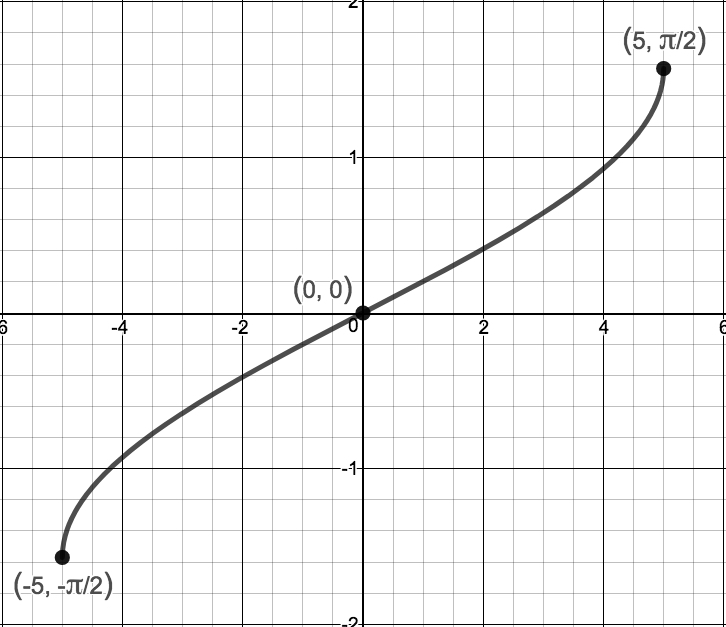
\includegraphics[height = 1.8in]{./TheInverseTrigonometricFunctionsGraphics/arccosgraph.jpg}

 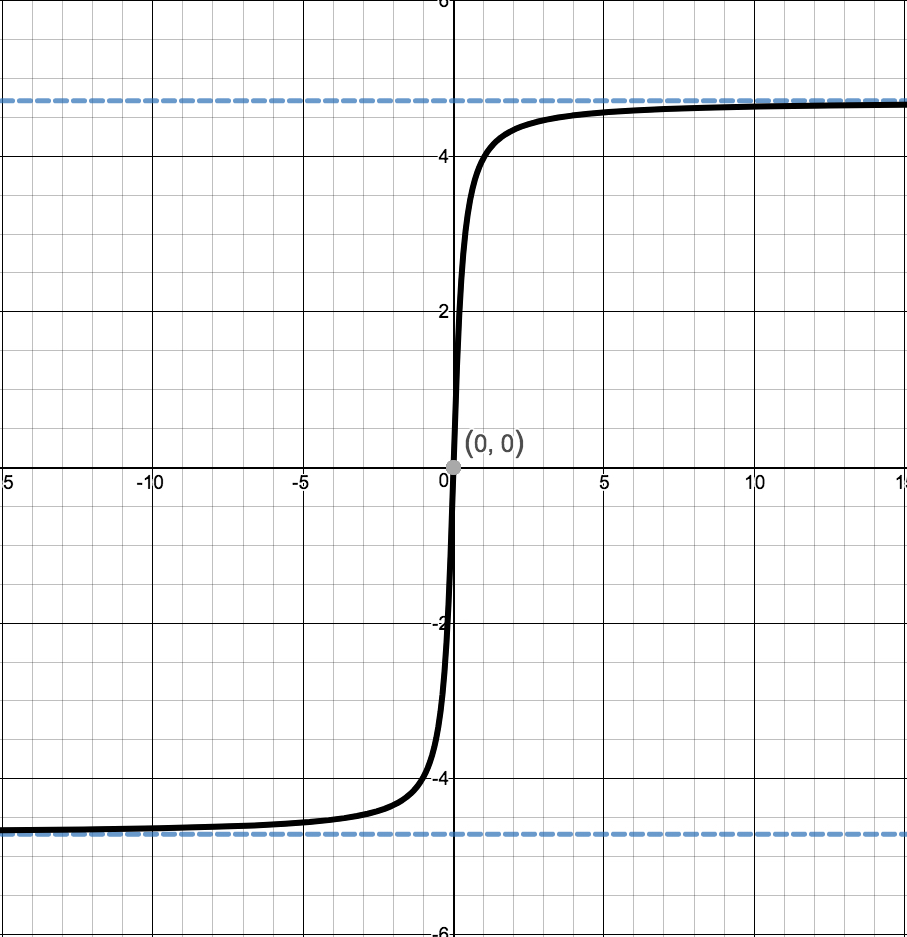
\includegraphics[height=1.81in]{./TheInverseTrigonometricFunctionsGraphics/arctangraph.jpg} 
 
 \end{multicols}

\begin{multicols}{2}

$y =f(x) = \frac{\pi}{2} - \arccos\left(\frac{x}{5}\right)$ 

$y = g(x) = 3\arctan\left(4x \right)$ \vphantom{$y =f(x) = \frac{\pi}{2} - \arccos\left(\frac{x}{5}\right)$ }

 \end{multicols}

\end{center}

\end{enumerate}

\end{enumerate}

\qed
\end{ex}

\subsection{Solving Equations Using the Inverse Trigonometric Functions.}

In Sections \ref{TheCircularFunctionsSineandCosine} and \ref{TheOtherCircularFunctions}, we learned how to solve equations like $\sin(\theta) = \frac{1}{2}$  and $\tan(t) = -1$. In each case, we ultimately appealed to the Unit Circle and relied on the fact that the answers corresponded to a set of `common angles' listed on page \pageref{commonanglesunitcircle}. 

\smallskip

 If, on the other hand, we had been asked to find all angles with $\sin(\theta) = \frac{1}{3}$ or solve $\tan(t) = -2$ for real numbers $t$, we would have been hard-pressed to do so.  With the introduction of the inverse trigonometric functions, however, we are now in a position to solve these equations. 
 
 \smallskip
 
 A good parallel to keep in mind is how the square root function can be used to solve certain quadratic equations.  The equation $x^2 = 4$ is a lot like  $\sin(\theta) = \frac{1}{2}$ in that it has friendly, `common value' answers  $x = \pm 2$.   The equation $x^2 = 7$, on the other hand, is a lot like $\sin(\theta) = \frac{1}{3}$.  We know there are answers, but we can't express them using `friendly' numbers.  
 
 \smallskip
 
 To solve $x^2 = 7$, we make use of the square root function (which is an inverse to $f(x) = x^2$ on a restricted domain) and write our answer as  $x = \pm \sqrt{7}$.  We need  the $\pm$ to  adjust for the fact that $\sqrt{7}$ is defined to be positive only, but we know we have two solutions, one positive and one negative.    Using a  calculator, we can certainly \textit{approximate} the values $\pm \sqrt{7}$,  but as far as exact answers go, we leave them as $x = \pm \sqrt{7}$.  
  
  \smallskip
  
In the same way, we will use the arcsine function (the inverse to the sine function on a restricted domain)  to solve $\sin(\theta) = \frac{1}{3}$.  However, we will need to adjust for the fact that there is more than one answer to this equation (infinitely many, in fact!)  As it turns out, we will be able to express every solution in terms of $\arcsin\left(\frac{1}{3}\right)$, as our next example illustrates.

\begin{ex}  \label{basicinverseeqns}  Solve the following equations.

\begin{enumerate}

\item  \label{basicinverseeqnssine} Find all angles $\theta$ for which $\sin(\theta) = \frac{1}{3}$.

\item \label{basicinverseeqnstangent} Find all real numbers $t$ for which $\tan(t) = -2$

\item  \label{basicinverseeqnssecant} Solve $\, \sec(x) = -\frac{5}{3} \,$ for $x$.

\end{enumerate}

{\bf Solution.}  

\begin{enumerate}

\item  If $\sin(\theta) = \frac{1}{3}$, then the terminal side of $\theta$, when plotted in standard position, intersects the Unit Circle at $y = \frac{1}{3}$.  Geometrically, we see that this happens at two places:  in Quadrant I and Quadrant II. 

\smallskip

If we let $\alpha$ denote the acute solution to the equation, then all the solutions to this equation in Quadrant I  are coterminal with $\alpha$, and $\alpha$ serves as the reference angle for all of the solutions to this equation in Quadrant II as seen below.

\smallskip

Since $\frac{1}{3}$ isn't the sine of any of the `common angles' we've encountered, we use the arcsine functions to express our answers.  By definition,  real number $t = \arcsin\left(\frac{1}{3}\right)$  $\sin(t) = \frac{1}{3}$ with $0 < t < \frac{\pi}{2}$.  

\smallskip

Hence, $\alpha = \arcsin\left(\frac{1}{3}\right)$ radians is an acute angle with $\sin(\alpha) = \frac{1}{3}$. Since all of the Quadrant I solutions $\theta$  are all coterminal with $\alpha$, we get $\theta = \alpha + 2\pi k  = \arcsin\left(\frac{1}{3}\right) + 2\pi k$ for integers $k$. 

\smallskip

 Turning our attention to Quadrant II, we get one solution to be $\pi - \alpha$.  Hence, the Quadrant II solutions are  $\theta = \pi - \alpha + 2\pi k = \pi - \arcsin\left(\frac{1}{3}\right) + 2\pi k$, for integers $k$.

\begin{tabular}{cc}

\begin{mfpic}[18]{-5}{5}{-5}{5}
\axes
\tlabel(5,-0.5){\scriptsize $x$}
\tlabel(0.25,5){\scriptsize $y$}
\tlabel(3.1,-0.75){\scriptsize $1$}
\tlabel(0.25,3.1){\scriptsize $1$}
\xmarks{-3 step 3 until 3}
\ymarks{-3, 1, 3}
\tlpointsep{4pt}
\axislabels{y}{{\scriptsize $\frac{1}{3}$} 1}
\drawcolor[gray]{0.7}
\circle{(0,0),3}
\drawcolor{black}
\arrow \parafcn{5, 20, 5}{2.75*dir(t)}
\penwd{1.25pt}
\arrow \reverse \arrow \polyline{(5,0), (0,0), (4.532, 2.113)}
\tlabel[cc](5.5, 0.61){\scriptsize $\alpha = \arcsin\left(\frac{1}{3}\right)$ radians}
\end{mfpic}

&

\hspace{0.25in}

\begin{mfpic}[18]{-5}{5}{-5}{5}
\axes
\tlabel(5,-0.5){\scriptsize $x$}
\tlabel(0.25,5){\scriptsize $y$}
\tlabel(3.1,-0.75){\scriptsize $1$}
\tlabel(0.25,3.1){\scriptsize $1$}
\xmarks{-3 step 3 until 3}
\ymarks{-3, 1, 3}
\tlpointsep{4pt}
\axislabels{y}{{\scriptsize $\frac{1}{3}$} 1}
\drawcolor[gray]{0.7}
\circle{(0,0),3}
\drawcolor{black}
\arrow \reverse \arrow \parafcn{160, 175, 5}{2.75*dir(t)}
\gclear \tlabelrect[cc](0, 2.5){\scriptsize \mbox{$\pi$}}
\arrow  \parafcn{5, 175, 5}{2*dir(t)}
\penwd{1.25pt}
\arrow \reverse \arrow \polyline{(5,0), (0,0), (-4.532, 2.113)}
\tlabel[cc](-3.45, 0.61){\scriptsize $\alpha$}
\end{mfpic} \\

\end{tabular}


\item The real number solutions to $\tan(t)=-2$  correspond to angles $\theta$  with $\tan(\theta) = -2$.  Since tangent is negative only in Quadrants II and IV, we focus our efforts there. 

\smallskip

The real number $t = \arctan(-2)$ satisfies $\tan(t)=-2$  and $-\frac{\pi}{2} < t < 0$.   If we let $\beta = \arctan(-2)$ radians, then all of the Quadrant IV solutions to  $\tan(\theta) = -2$  are coterminal with $\beta$. 

\smallskip

Moreover, as seen below on the right, the solutions from Quadrant II differ by exactly $\pi$ units from the solutions in Quadrant IV (recall, the period  of the tangent function is $\pi$.)  Hence, all of the  solutions to $\tan(\theta) = -2$ are of the form $\theta = \beta + \pi k = \arctan(-2) + \pi k$ for some integer $k$.   Switching back to the variable $t$,  we record our final answer to $\tan(t) = -2$ as $t = \arctan(-2) + \pi k$ for integers $k$.

\begin{tabular}{cc}

\begin{mfpic}[18]{-5}{5}{-5}{5}
\axes
\tlabel(5,-0.5){\scriptsize $x$}
\tlabel(0.25,5){\scriptsize $y$}
\tlabel(3.1,0.25){\scriptsize $1$}
\tlabel(0.25,3.1){\scriptsize $1$}
\xmarks{-3 step 3 until 3}
\ymarks{-3 step 3 until 3}
\drawcolor[gray]{0.7}
\circle{(0,0),3}
\drawcolor{black}
\arrow \parafcn{355, 305, -5}{1.5*dir(t)}
\gclear \tlabelrect[cc](4, -1){\scriptsize $\beta = \arctan(-2)$ radians}
\penwd{1.25pt}
\arrow \reverse \arrow \polyline{(5,0), (0,0), (2.5, -4.3301)}
\end{mfpic}

&

\hspace{.25in}


\begin{mfpic}[18]{-5}{5}{-5}{5}
\axes
\tlabel(5,-0.5){\scriptsize $x$}
\tlabel(0.25,5){\scriptsize $y$}
\tlabel(3.1,0.25){\scriptsize $1$}
\tlabel(0.25,3.1){\scriptsize $1$}
\xmarks{-3 step 3 until 3}
\ymarks{-3 step 3 until 3}
\drawcolor[gray]{0.7}
\circle{(0,0),3}
\drawcolor{black}
\arrow \parafcn{355, 305, -5}{1.5*dir(t)}
\arrow \reverse \arrow \parafcn{125, 295, 5}{1.5*dir(t)}
\tlabel[cc](-2, -1){\scriptsize $\pi$}
\tlabel[cc](2, -1){\scriptsize $\beta$}
\penwd{1.25pt}
\arrow \reverse \arrow \polyline{(5,0), (0,0), (-2.5, 4.3301)}
\arrow \reverse \arrow \polyline{(5,0), (0,0), (2.5, -4.3301)}
\end{mfpic} \\

\end{tabular}

\smallskip

Another tact we could have taken to solve this problem is to use reference angles.  Consider the (angle) equation: $\tan(\theta) = -2$.  If we let $\alpha$ be the reference angle for the solutions $\theta$, we know $\alpha$ is an acute angle with $\tan(\alpha) = 2$.  

\smallskip

By definition, the real number $t = \arctan(2)$ satisfies $0 < t < \frac{\pi}{2}$ with $\tan(t) = 2$.  Hence, the angle $\alpha = \arctan(2)$ radians is the reference angle for our solutions to $\tan(\theta) = -2$.  

\smallskip

Adjusting for quadrants, we get our answers to $\tan(\theta) = -2$ are  $\theta = - \alpha + \pi k = -\arctan(2) + \pi k$ for integers $k$.   Again, we cosmetically change the variable from $\theta$ back to $t$ so our answer to $\tan(t) = -2$ is $t = -\arctan(2) + \pi k$.  Thanks to the odd property of arctangent,  $\arctan(-2) = -\arctan(2)$ and we see this family of solutions is identical to what we obtained earlier.

\begin{tabular}{cc}

\begin{mfpic}[18]{-5}{5}{-5}{5}
\axes
\tlabel(5,-0.5){\scriptsize $x$}
\tlabel(0.25,5){\scriptsize $y$}
\tlabel(3.1,-0.25){\scriptsize $1$}
\tlabel(0.25,3.1){\scriptsize $1$}
\xmarks{-3 step 3 until 3}
\ymarks{-3 step 3 until 3}
\drawcolor[gray]{0.7}
\circle{(0,0),3}
\drawcolor{black}
\arrow \parafcn{5, 55, 5}{1.5*dir(t)}
\gclear \tlabelrect[cc](4, 1){\scriptsize $\alpha = \arctan(2)$ radians}
\penwd{1.25pt}
\arrow \reverse \arrow \polyline{(5,0), (0,0), (2.5, 4.3301)}
\end{mfpic}

&

\hspace{.25in}


\begin{mfpic}[18]{-5}{5}{-5}{5}
\axes
\tlabel(5,-0.5){\scriptsize $x$}
\tlabel(0.25,5){\scriptsize $y$}
\tlabel(3.1,-0.25){\scriptsize $1$}
\tlabel(0.25,3.1){\scriptsize $1$}
\xmarks{-3 step 3 until 3}
\ymarks{-3 step 3 until 3}
\drawcolor[gray]{0.7}
\circle{(0,0),3}
\drawcolor{black}
\arrow \reverse \arrow \parafcn{355, 305, -5}{1.5*dir(t)}
\arrow \reverse \arrow \parafcn{125, 295, 5}{1.5*dir(t)}
\tlabel[cc](-2, -1){\scriptsize $\pi$}
\tlabel[cc](2, -1){\scriptsize $\alpha$}
\penwd{1.25pt}
\arrow \reverse \arrow \polyline{(5,0), (0,0), (-2.5, 4.3301)}
\arrow \reverse \arrow \polyline{(5,0), (0,0), (2.5, -4.3301)}
\end{mfpic} \\

\end{tabular}



\item  In the last equation, $\sec(x) = -\frac{5}{3}$, we are not told whether or not $x$ represents an angle or a real number.  This isn't really much of an issue, since we attack both problems the same way.  

\smallskip

Taking a cue from our work in Section \ref{TheOtherCircularFunctions} and use a Reciprocal Identity to convert the equation $\sec(x) = -\frac{5}{3}$ to   $\cos(x) = -\frac{3}{5}$.    Thinking geometrically,  we are looking for angles $\theta$ with  $\cos(\theta) = -\frac{3}{5}$.  Since $\cos(\theta) < 0$, we are looking for solutions in  Quadrants II and III.   Since $-\frac{3}{5}$ isn't  the cosine of any of the `common angles', we'll need to express our solutions in terms of the arccosine function.  


\begin{tabular}{cc}


\begin{mfpic}[18]{-5}{5}{-5}{5}
\axes
\tlabel(5,-0.5){\scriptsize $x$}
\tlabel(0.25,5){\scriptsize $y$}
\tlabel(3.1,-0.75){\scriptsize $1$}
\tlabel(0.25,3.1){\scriptsize $1$}
\xmarks{-3 step 3 until 3}
\ymarks{-3 step 3 until 3}
\drawcolor[gray]{0.7}
\circle{(0,0),3}
\drawcolor{black}
\arrow \parafcn{5, 115, 5}{1.5*dir(t)}
\gclear \tlabelrect[cc](4, 1.5){\scriptsize $\beta = \arccos\left(-\frac{3}{5}\right)$ radians}
\penwd{1.25pt}
\arrow \reverse \arrow \polyline{(5,0), (0,0), (-2.5, 4.3301)}
\end{mfpic}
&

\hspace{-.15in}

\begin{mfpic}[18]{-5}{5}{-5}{5}
\axes
\tlabel(5,-0.5){\scriptsize $x$}
\tlabel(0.25,5){\scriptsize $y$}
\tlabel(3.1,-0.75){\scriptsize $1$}
\tlabel(0.25,3.1){\scriptsize $1$}
\xmarks{-3 step 3 until 3}
\ymarks{-3 step 3 until 3}
\drawcolor[gray]{0.7}
\circle{(0,0),3}
\drawcolor{black}
\arrow \dotted \parafcn{5, 115, 5}{1.5*dir(t)}
\gclear \tlabelrect[cc](4, 1.5){\scriptsize $\beta = \arccos\left(-\frac{3}{5}\right)$ radians}
\arrow \parafcn{355, 245, -5}{1.5*dir(t)}
\dashed \polyline{ (0,0), (-2.5, 4.3301)}
\gclear \tlabelrect[cc](4, -1.5){\scriptsize $-\beta = -\arccos\left(-\frac{3}{5}\right)$ radians}
\penwd{1.25pt}
\arrow \reverse \arrow \polyline{(5,0), (0,0), (-2.5, -4.3301)}
\end{mfpic} \qed \\


\end{tabular}


The real number $t = \arccos\left(-\frac{3}{5}\right)$ is defined so that $\frac{\pi}{2} < t < \pi$ with $\cos(t) = -\frac{3}{5}$.  Hence, the angle $\beta = \arccos\left(-\frac{3}{5}\right)$ radians is a Quadrant II angle which satisfies $\cos(\beta) = -\frac{3}{5}$. To obtain a Quadrant III angle solution, we may simply use $-\beta = -\arccos\left(-\frac{3}{5}\right)$ as seen above on the right.

\smallskip

Since all angle solutions are coterminal with $\beta$ or $-\beta$, we get our solutions to $\cos(\theta) = -\frac{3}{5}$ to be $\theta = \beta + 2\pi k = \arccos\left(-\frac{3}{5}\right) + 2\pi k$ or $\theta = -\beta + 2\pi k = -\arccos\left(-\frac{3}{5}\right) + 2\pi k$ for integers $k$.  

\smallskip

Switching back to the variable $x$,  we record our final answer to $\sec(x) = -\frac{5}{3}$ as $x = \arccos\left(-\frac{3}{5}\right) + 2\pi k$ or $x = -\arccos\left(-\frac{3}{5}\right) + 2\pi k$ for integers $k$.


\smallskip

As with the previous problem, we can approach solving  $\cos(\theta) = -\frac{3}{5}$ using reference angles.  Letting $\alpha$ represent the reference angle for the solutions $\theta$, we know $\alpha$ is an acute angle with $\cos(\alpha) = \frac{3}{5}$.

\smallskip

We know the real number $t = \arccos\left( \frac{3}{5} \right)$ satisfies $\cos(t) = \frac{3}{5}$ and $0 < t < \frac{\pi}{2}$, hence $\alpha = \arccos\left( \frac{3}{5} \right)$ radians is the reference angle for the solutions to  $\cos(\theta) = -\frac{3}{5}$.

\smallskip

Hence, the Quadrant II solutions to $\cos(\theta) = -\frac{3}{5}$ are $\theta = \pi - \alpha + 2\pi k = \pi -  \arccos\left( \frac{3}{5} \right) + 2\pi k$  while the Quadrant IV solutions to $\cos(\theta) = -\frac{3}{5}$ are $\theta = \pi + \alpha + 2\pi k = \pi + \arccos\left( \frac{3}{5} \right) + 2\pi k$ for integers $k$.

\begin{tabular}{cc}


\begin{mfpic}[18]{-5}{5}{-5}{5}
\axes
\tlabel(5,-0.5){\scriptsize $x$}
\tlabel(0.25,5){\scriptsize $y$}
\tlabel(3.1,-0.75){\scriptsize $1$}
\tlabel(0.25,3.1){\scriptsize $1$}
\xmarks{-3 step 3 until 3}
\ymarks{-3 step 3 until 3}
\drawcolor[gray]{0.7}
\circle{(0,0),3}
\drawcolor{black}
\arrow \parafcn{5, 55, 5}{1.5*dir(t)}
\gclear \tlabelrect[cc](4, 1.5){\scriptsize $\alpha = \arccos\left(\frac{3}{5}\right)$ radians}
\penwd{1.25pt}
\arrow \reverse \arrow \polyline{(5,0), (0,0), (2.5, 4.3301)}
\end{mfpic}
&

\hspace{-.15in}

\begin{mfpic}[18]{-5}{5}{-5}{5}
\axes
\tlabel(5,-0.5){\scriptsize $x$}
\tlabel(0.25,5){\scriptsize $y$}
\tlabel(3.1,-0.75){\scriptsize $1$}
%\tlabel(0.25,3.1){\scriptsize $1$}
\xmarks{-3 step 3 until 3}
\ymarks{-3 step 3 until 3}
\drawcolor[gray]{0.7}
\circle{(0,0),3}
\drawcolor{black}
\arrow \parafcn{5, 115, 5}{1.25*dir(t)}
\gclear \tlabelrect[cc](0.75, 3){\scriptsize $\pi - \arccos\left(\frac{3}{5}\right)$ radians}
\arrow \parafcn{5, 235, -5}{dir(t)}
\gclear \tlabelrect[cc](0.75, -3){\scriptsize $\pi + \arccos\left(-\frac{3}{5}\right)$ radians}
\arrow \reverse \arrow \parafcn{185, 235, 5}{1.5*dir(t)}
\gclear \tlabelrect[cc](-4, 1){\scriptsize $\alpha = \arccos\left(\frac{3}{5}\right)$ radians}
\arrow \reverse \arrow \parafcn{125, 175, 5}{1.5*dir(t)}
\gclear \tlabelrect[cc](-4, -1){\scriptsize $\alpha = \arccos\left(\frac{3}{5}\right)$ radians}
\penwd{1.25pt}
\arrow \reverse \arrow \polyline{(5,0), (0,0), (-2.5, -4.3301)}
\arrow \reverse \arrow  \polyline{ (5,0), (0,0), (-2.5, 4.3301)}
\end{mfpic} \qed \\


\end{tabular}

Shifting back to the variable $x$, we get our solution to $\sec(x) = -\frac{5}{3}$ are $x =  \pi -  \arccos\left( \frac{3}{5} \right) + 2\pi k$ or $x = \pi + \arccos\left( \frac{3}{5} \right) + 2\pi k$ for integers $k$.  While these certainly look quite different than what we obtained before, $x = \arccos\left(-\frac{3}{5}\right) + 2\pi k$ or $x = -\arccos\left(-\frac{3}{5}\right) + 2\pi k$ for integers $k$, they are, in fact, equivalent.  To show this, we start with $\arccos\left(-\frac{3}{5} \right) = \pi - \arccos\left(\frac{3}{5} \right)$ and begin writing out specific solutions from each family by choosing specific values of $k$.  We leave these details to the reader.  \qed


\end{enumerate}

\end{ex}

\smallskip

We close this section with one last sinusoid example.

\begin{ex}  \label{expandedsinusoidinverseex}  Consider the function $f(t) = 3\cos(6t) -4 \sin(6t)$. Find a formula for $f(t)$:

\begin{enumerate}

\item  in the form $C(t) = A \cos(\omega t + \phi) + B$ for $\omega > 0$

\item  in the form $S(t) = A \sin(\omega t + \phi) + B$ for $\omega > 0$

\end{enumerate}

{\bf Solution.}  

\begin{enumerate}

\item As in Example \ref{expandedsinusoidex1}, we compare the expanded form of $C(t) = A \cos(\omega t) \cos(\phi) - A \sin(\omega t) \sin(\phi) + B$ with $f(t) = 3\cos(6t) -4 \sin(6t)$. We identify $\omega = 6$ and $B = 0$ and by equating coefficients of  $\cos(6t)$ and $\sin(6t)$  get the two equations: $A \cos(\phi) = 3$ and $A \sin(\phi) = 4$.

\smallskip

Using the Pythagorean Identity to eliminate $\phi$, we get $A^2 = (A \cos(\phi))^2 + (A \sin(\phi))^2 = 3^2 + 4^2 = 25$.  We choose $A = 5$ and work to find the phase angle $\phi$.

\smallskip

Substituting $A = 5$ into our two equations relating $A$ and $\phi$, we get $5 \cos(\phi) = 3$, or $\cos(\phi) = \frac{3}{5}$  and $5 \sin(\phi) = 4$, so $\sin(\phi) = \frac{4}{5}$.  Since both $\sin(\phi)$ and $\cos(\phi)$ are positive, we know $\phi$ is a Quadrant I angle.  However, since neither the sine nor cosine value of $\phi$ corresponds to a common angle, we need to express $\phi$ in terms of either an arcsine or arccosine.

\smallskip

Since the real number $t = \arccos\left(\frac{3}{5}\right)$ satisfies $\cos(t) = \frac{3}{5}$ and $0 < t < \frac{\pi}{2}$, we know the angle $\phi = \arccos\left(\frac{3}{5}\right)$ radians is an acute (Quadrant I) angle which satisfies $\cos(\phi) = \frac{3}{5}$.  Hence, we can take $\phi = \arccos\left(\frac{3}{5}\right)$ and write $f(t) = 5 \cos\left(6t + \arccos\left(\frac{3}{5}\right) \right)$.

\smallskip

In addition, the real number $t = \arcsin\left(\frac{4}{5}\right)$ satisfies $\sin(t) = \frac{4}{5}$ and $0 < t < \frac{\pi}{2}$.  Hence $\phi = \arcsin\left(\frac{4}{5}\right)$ radians is Quadrant I angle with  $\sin(\phi) = \frac{4}{5}$.  This means we could also take $\phi = \arcsin\left(\frac{4}{5}\right)$ and write $f(t) = 5 \cos\left(6t + \arcsin\left(\frac{4}{5}\right) \right)$.  (We could also express $\phi$ in terms of arctangents, if we wanted!)

\smallskip

We leave it to the reader to verify (both) solutions analytically and graphically.


\item Once again, we equate the expanded form of $S(t) = A \sin(\omega t) \cos(\phi) + A \cos(\omega t) \sin(\phi) + B$ with $f(t) = 3\cos(6t) -4 \sin(6t)$. Once again, we get  $\omega = 6$ and $B = 0$.  Here, our two equations for $A$ and $\phi$ are $A \cos(\phi) = -4$ and $A \sin(\phi) = 3$.

\smallskip

As before, we get $A^2 = (A \cos(\phi))^2 + (A \sin(\phi))^2 = (-4)^2 + 3^2 = 25$, and we choose $A = 5$. Our equations for $\phi$ become:  $\cos(\phi) = -\frac{4}{5}$ and $\sin(\phi) = \frac{3}{5}$.  Since $\cos(\phi)<0$ but $\sin(\phi) > 0$, we know $\phi$ is a Quadrant II angle. As before, since neither the sine nor cosine value of $\phi$ corresponds to a common angle, we need to express $\phi$ in terms of either an arcsine or arccosine.

\smallskip

Here, we opt to use the arccosine function, since the range of arccosine, $[0, \pi]$ covers Quadrant II.   From  $\cos(\phi) = -\frac{4}{5}$ , we get $\phi = \arccos\left(-\frac{4}{5}\right)$, so $f(t) = 5 \sin\left(6t + \arccos\left(-\frac{4}{5}\right) \right)$.  

\smallskip

Had we chosen to work with arcsines, we would need a Quadrant II solution to $\sin(\phi) = \frac{3}{5}$.  Going through the usual machinations, we arrive at $\phi = \pi - \arcsin\left( \frac{3}{5} \right)$.  Hence, an alternative form of our answer is $f(t) = 5 \sin \left( 6t +  \pi - \arcsin\left( \frac{3}{5} \right) \right)$.  We leave the checks to the reader.  \qed

\end{enumerate}


\end{ex}


\newpage
\subsection{Exercises}

%% SKIPPED %% \input{ExercisesforTheInverseTrigonometricFunctions}

\closegraphsfile

\end{document}
